\chapter{Modellbildung} \label{ch_Modellbildung}
Die Modellbildung hat das Ziel, das dynamische Verhalten des Heliostatenfeldes und des Receivers am Solarturm in Jülich zu beschreiben.
Zu diesem Zweck wird das in Kapitel \ref{sec_Ausgangszustand} vorgestellte Modell eines Absorbercups um den Einfluss des Gebläses im Receiver auf ein thermisches Teilmodell erweitert.
Weiterhin wird ein optisches Teilmodell zur Beschreibung der solaren Einstrahlung, der Heliostaten und deren Brennflecken auf dem Receiver eingeführt.
Abschließend wird die Modellbildung durch die Kopplung der beiden Teilsysteme vervollständigt.

\section{Thermisches Teilmodell} \label{sec_thermischesModell}
Zur Regelung des Massenstroms im Receiver müssen die Gebläse und Ventile im Luftkreislauf angesteuert werden.
Gemäß \cite[S.10ff]{DissGall} existieren zwei Gebläse/Ventil-Kombinationen, die für den Luftstrom im Solarturm verantwortlich sind.
Durch diese kann der Anteil der Luft verändert werden, der durch den Receiver, den Wärmespeicher oder den Dampfkraftprozess strömt.
In einer integrierten zweistufigen Regelung werden abhängig von einem Einstellwert Ventilstellung und Gebläsedrehzahl angepasst, um einen gewünschten Luftmassenstrom zu erreichen.
Im Rahmen dieser Arbeit wird lediglich die Gebläse/Ventil-Kombination geregelt, die den Massenstrom im Receiver einstellt, da die weitere Verwendung der Luft zur Stromerzeugung oder Speicherung nicht betrachtet wird.

\subsection{Analyse der Lüftungsdynamik} \label{subsec_AnalyseLüftungsDyn}
Durch die Wechselwirkung von Ventil und Gebläse entsteht bei einem Sprung des Einstellwertes eine gedämpft schwingende Anpassung des Luftstroms.
Dieses Verhalten zeigt die in Abbildung \ref{fig_LuftstromSolarturm} dargestellte Messung am Solarturm vom 07.08.2022.
Auf der rechten Achse ist der Einstellwert der Gebläse/Ventil-Kombination in Normkubikmetern pro Stunde erkennbar, während links der zugehörige Massenstrom in Kilogramm pro Sekunde aufgetragen ist.
Es ist zu erwähnen, dass die Änderung des Luftmassenstroms um 12:20 Uhr Störungen unterlag. \pagebreak

\begin{figure}[h!]
    \centering
    \setlength{\fboxsep}{1pt}
    \setlength{\fboxrule}{1pt}
    \fbox{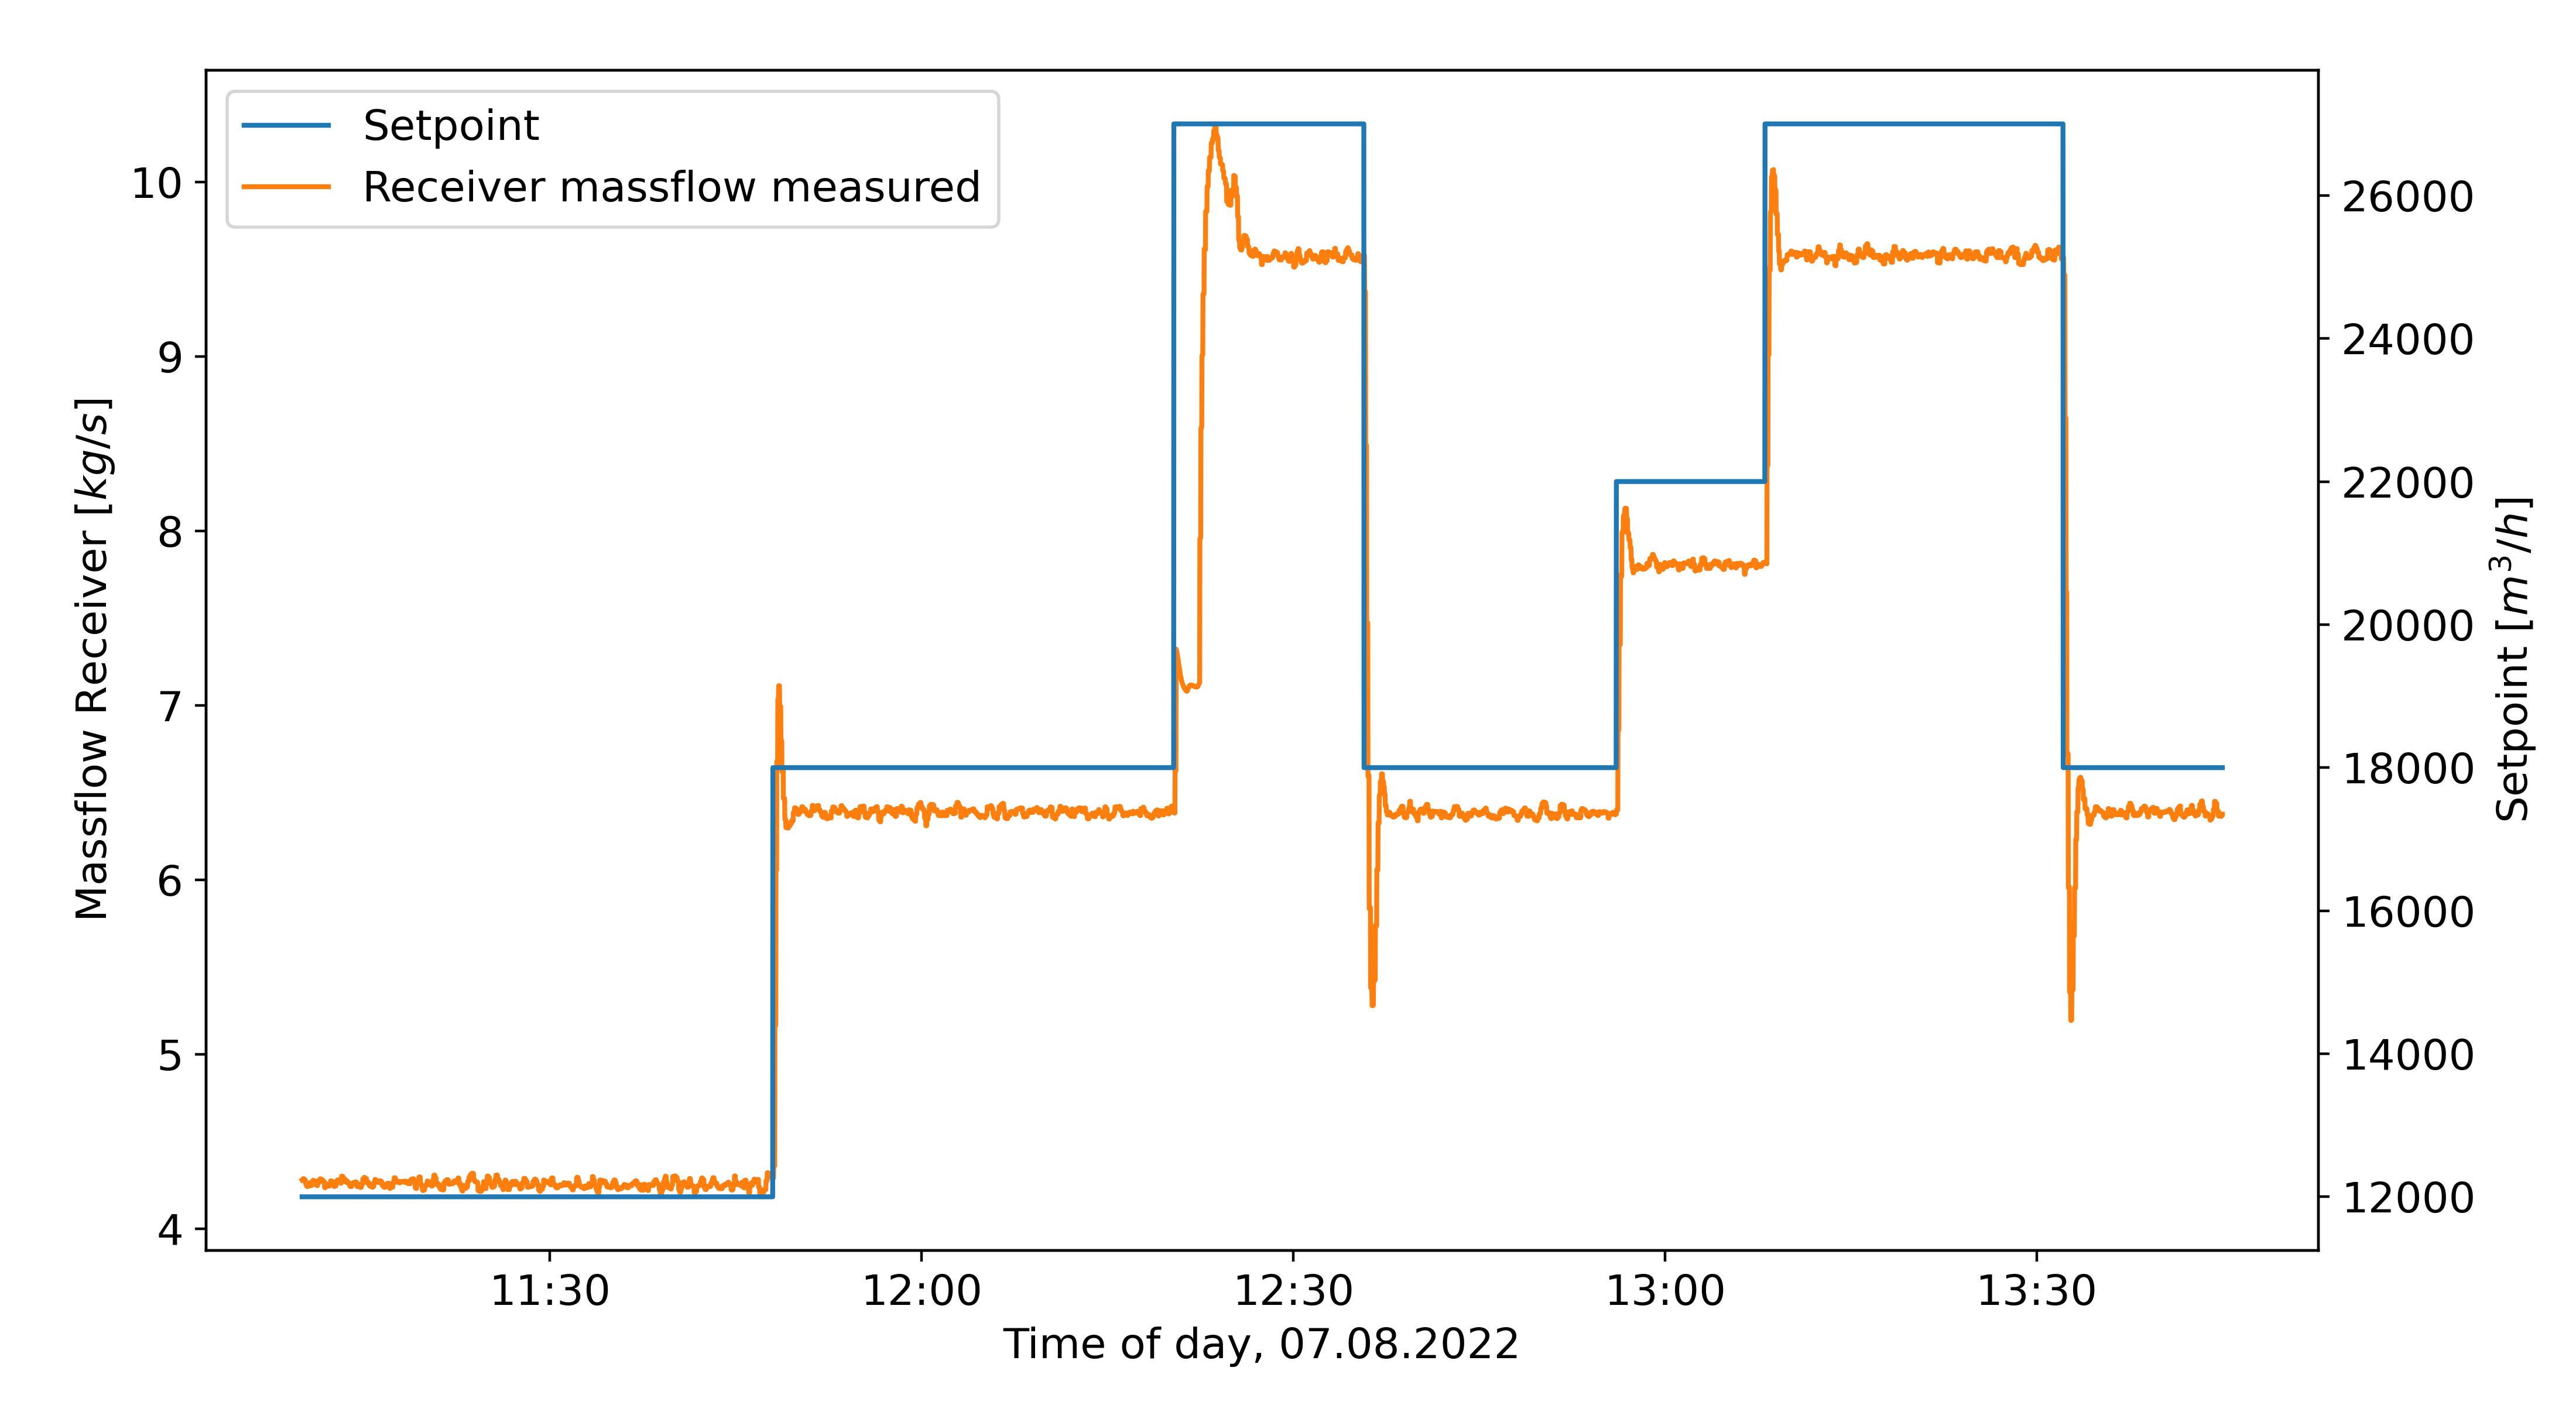
\includegraphics[width=0.95\textwidth]{C:/Users/gesc_ma/VSCode MPC Projekt/dynaovrcontroller/dynaovrcontroller/aimpoint_control_scenarios/plots/12_fan_parameter/measured_fan_data.png}}
\caption[Luftstrommessung für unterschiedliche Einstellwerte am Solarturm Jülich\linebreak (07.08.2022)]{Luftstrommessung für unterschiedliche Einstellwerte am Solarturm Jülich\linebreak (07.08.2022)}
    \label{fig_LuftstromSolarturm}
\end{figure}

Um die Veränderung des Luftmassenstroms bei Einstellwertänderungen simulativ annähern zu können, wird dieser durch ein PT2-Verhalten modelliert.
Ein solches Verhalten zeigt Abbildung \ref{fig_SprungantwortSymbolisch}.
Die zugehörige Differentialgleichung beschreibt die Änderung der Ausgangsgröße~$y$ und deren Ableitungen bei Änderung der Eingangsgröße $u$.
Gleichung \ref{eq_ÜbertrgaungsfunktionPT2} definiert die\linebreak allgemeine Differentialgleichung eines PT2-Gliedes in Abhängigkeit von der\linebreak Zeit $t$ \cite[S.200]{Lunze}\cite[S.60]{ProfMueller}.

\begin{equation} \label{eq_ÜbertrgaungsfunktionPT2}
K_p u(t) = T^2 \ddot{y}(t)+2 D T \dot{y}(t)+y(t)
\end{equation}
% \centerline{\small{\textsf{\textbf{Formel \ref{eq_Label}:}} Beschriftung}}
\myequations{\quad Übertragungsfunktion eines schwingungsfähigen PT2 Gliedes}

Zur Beschreibung des PT2-Verhaltens der Lüftungsdynamik werden die drei unbekannten Größen aus Gleichung \ref{eq_ÜbertrgaungsfunktionPT2} ermittelt.
Dies sind die Zeitkonstante $T$ zur Beschreibung der Geschwindigkeit der Veränderung, die Dämpfungskonstante $D$, die das Einschwingverhalten beschreibt, und der Proportionalitätsfaktor $K_p$.
Anhand Abbildung \ref{fig_SprungantwortSymbolisch} werden die Messgrößen einer Einheitssprungantwort $h(t)$ identifiziert, die zur Bestimmung dieser Größen benötigt werden.\pagebreak

\begin{figure}[h!]
    \centering
    \setlength{\fboxsep}{1pt}
    \setlength{\fboxrule}{1pt}
    \fbox{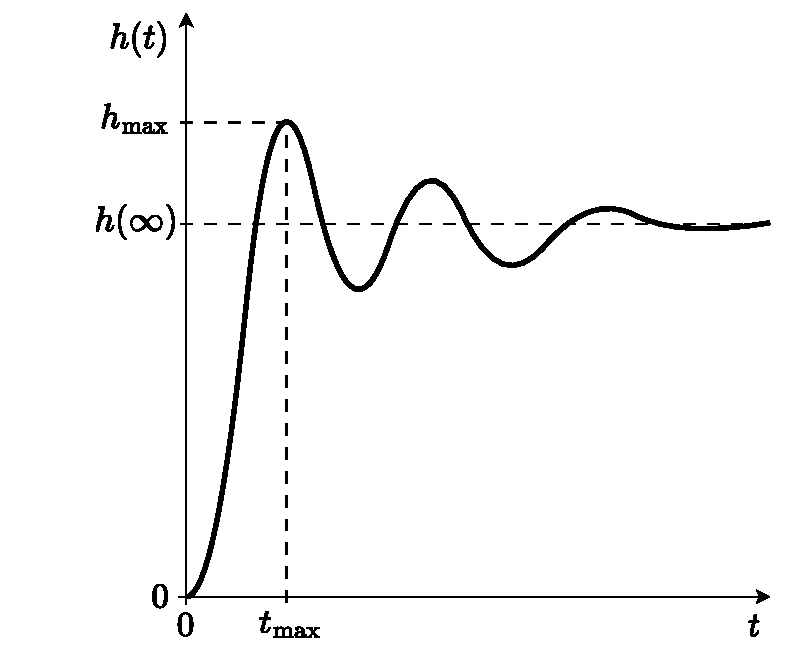
\includegraphics[width=0.55\textwidth]{fig/Sprungantwort}}
    \caption[Exemplarische Einheitssprungantwort eines PT2-Gliedes]{Exemplarische Einheitssprungantwort eines PT2-Gliedes (nach \cite[S.60]{ProfMueller})}
    \label{fig_SprungantwortSymbolisch}
\end{figure}

Der Proportionalitätsfaktor $K_p$ ergibt sich unter Betrachtung des stationären Verhaltens $h(t\rightarrow \infty)$ gemäß Gleichung \ref{eq_BerechnungKP}:

\begin{equation} \label{eq_BerechnungKP}
    K_p = \frac{h(t\rightarrow \infty) - h(t=0)}{\Delta u}
\end{equation}
% \centerline{\small{\textsf{\textbf{Formel \ref{eq_Label}:}} Beschriftung}}
\myequations{\quad Berechnung des Proportionalitätsfaktors $K_p$ bei PT2-Gliedern}

Für schwingfähige Systeme lässt sich der Dämpfungsfaktor $D$ aus der relativen Überschwingweite $os$ der Sprungantwort ermitteln.
Es gilt:
\begin{equation} \label{eq_BerechnungD}
    D = \frac{\ln \left(\frac{1}{os}\right)}{\sqrt{\pi^2+\left(\ln\left[\frac{1}{os}\right]\right)^2}},
\end{equation}
% \centerline{\small{\textsf{\textbf{Formel \ref{eq_Label}:}} Beschriftung}}
\myequations{\quad Berechnung des Dämpfungsfaktors $D$ bei PT2-Gliedern}

\vspace*{-\baselineskip}mit

\begin{equation} \label{eq_overshoot}
    os = \frac{h_{\mathrm{max}}-h(t\rightarrow \infty)}{h(t\rightarrow \infty)}.
\end{equation}
% \centerline{\small{\textsf{\textbf{Formel \ref{eq_Label}:}} Beschriftung}}
\myequations{\quad Berechnung der relativen Überschwingweite $os$}

Die Zeitkonstante eines PT2-Gliedes wird durch Berücksichtigung des Zeitpunktes $t_{\mathrm{max}}$ bestimmt, zu dem das maximale Überschwingen $h_{\mathrm{max}}$ auftritt (vgl. Abbildung \ref{fig_SprungantwortSymbolisch}).
Sie berechnet sich wie folgt:

\begin{equation} \label{eq_BerechnungT}
    T = \frac{t_{\mathrm{max}} \cdot \sqrt{1-D^2}}{\pi}
\end{equation}
% \centerline{\small{\textsf{\textbf{Formel \ref{eq_Label}:}} Beschriftung}}
\myequations{\quad Berechnung der Zeitkonstante $T$ bei PT2-Gliedern}


\subsection{Modellierung der Lüftungsdynamik} \label{subsec_BeschreibungLüftungsDyn}
Unter Betrachtung der störungsfreien Einstellwertänderungen aus Abbildung \ref{fig_LuftstromSolarturm} werden die konkreten Parameter der Lüftungsdynamik bestimmt.
Dazu werden die drei Parameter $K_p$, $D$ und $T$ für jeden in Abbildung \ref{fig_LuftstromSolarturm} erkennbaren Betriebspunktwechsel separat errechnet und anschließend gemittelt.
Es ergeben sich $K_p = \SI{3.55e-4}{\kilo\gram\hour\per\second\per\metre\cubed}$, $T = \SI{11.60}{\second}$ und\linebreak $D = \SI{0.35}{}$.
Die Genauigkeit dieser Berechnungen zeigt nachfolgend Abbildung \ref{fig_LuftstromplusSimulativ}, in der erkennbar ist, dass das simulierte Verhalten des Massenstroms mit den Messwerten übereinstimmt.
Die Wurzel des mittleren quadratischen Fehlers (der \textit{RMSE}) liegt über den Simulationszeitraum unter Ausschluss der invaliden Daten zwischen 12:20 Uhr und 12:40 Uhr bei $\SI{0.043}{\kilo\gram\per\second}$.

\begin{figure}[h!]
    \centering
    \setlength{\fboxsep}{1pt}
    \setlength{\fboxrule}{1pt}
    \fbox{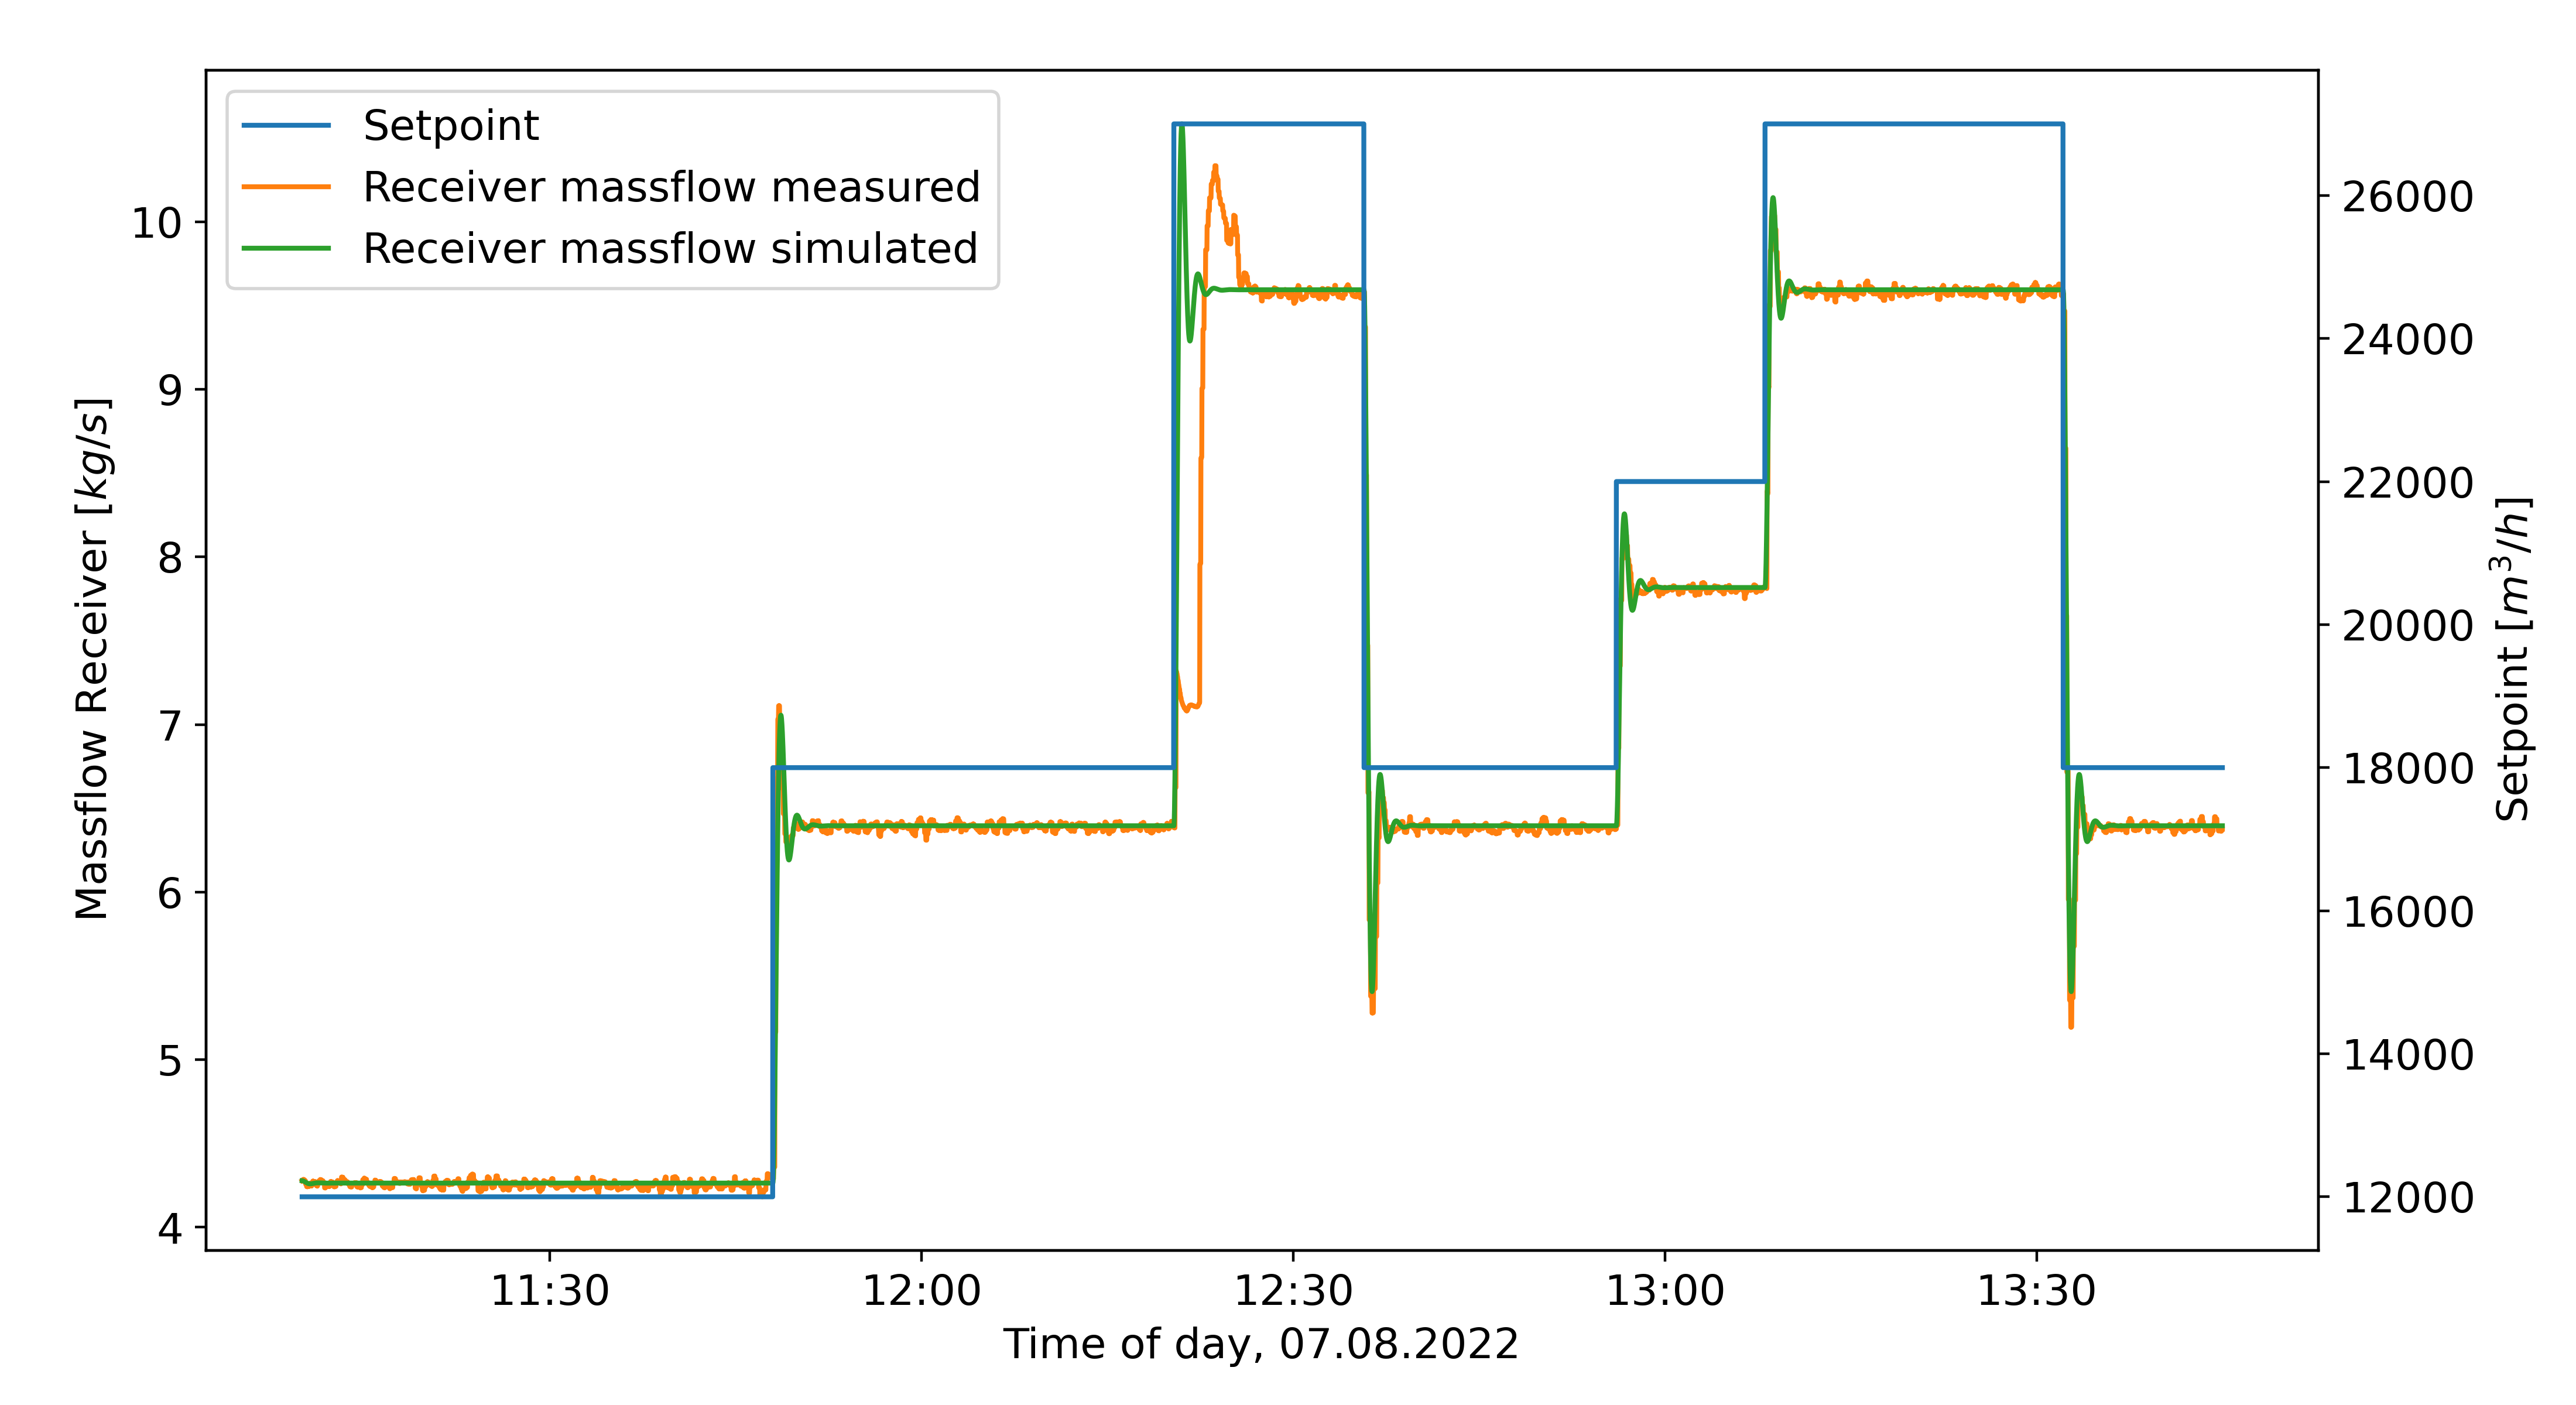
\includegraphics[width=0.95\textwidth]{C:/Users/gesc_ma/VSCode MPC Projekt/dynaovrcontroller/dynaovrcontroller/aimpoint_control_scenarios/plots/12_fan_parameter/fan_parameter_fitting.png}}
    \caption[Vergleich der simulierten Massenströme mit den Messwerten vom 07.08.2022]{Vergleich der simulierten Massenströme mit den Messwerten vom 07.08.2022}
    \label{fig_LuftstromplusSimulativ}
\end{figure}

Die Annäherung des Luftmassenstroms durch dieses PT2 Verhalten ist nur im Rahmen des zulässigen Betriebsbereiches des Solarturms für den Massenstrom valide.
Er ergibt sich gemäß dem Betriebshandbuch des Herstellers zu $\SIrange{2.93}{11.7}{\kilo\gram\per\second}$ \cite[S.28]{HandbuchJülich}.
Daraus folgt der für den Einstellwert zulässige Bereich von $\SIrange{8254}{32957}{\metre\cubed\per\hour}$.

Konkret ergibt sich Gleichung \ref{eq_ÜbertrgaungsfunktionPT2} mit der Ausgangsgröße $y$ als Luftmassenstrom $\MDotReceiver$ zu der in Gleichung \ref{eq_GesamtDGL} dargestellten Differentialgleichung zweiter Ordnung.
Dabei steht $u_{\mathrm{setpoint}}(t)$ für den zeitlich veränderlichen Einstellwert.

\begin{equation} \label{eq_GesamtDGL}
K_p u_{\mathrm{setpoint}}(t) = T^2 \frac{d^2\MDotReceiver}{dt^2} + 2 D T \frac{d\MDotReceiver}{dt} + \MDotReceiver
\end{equation}
% \centerline{\small{\textsf{\textbf{Formel \ref{eq_Label}:}} Beschriftung}}
\myequations{\quad Differentialgleichung der Lüftungsdynamik}

Aufgrund des geringeren Berechnungsaufwandes bei der numerischen Lösung von\linebreak Differentialgleichungen erster Ordnung im Vergleich zu solchen mit höherer Ord-\linebreak nung \cite[S.138-139]{Gausch}\cite[S.241ff]{Howell}, wird Gleichung \ref{eq_GesamtDGL} in zwei Differentialgleichungen erster Ordnung umgeschrieben.
Dazu werden zwei Zustände eingeführt: einer für den Massenstrom $\MDotReceiver$ und einer für dessen zeitliche Änderung $\ddot{m}_{\mathrm{rec}}$.
\begin{equation} \label{eq_Einführtungstates}
\begin{gathered}
    x_1 = \MDotReceiver\\
    x_2 = \ddot{m}_{\mathrm{rec}}
\end{gathered}
\end{equation}
% \centerline{\small{\textsf{\textbf{Formel \ref{eq_Label}:}} Beschriftung}}
\myequations{\quad Einführung des Massenstroms und dessen Ableitung als Systemzustände}

Die Differentialgleichungen ergiben sich zu:
\begin{equation} \label{eq_DGLsMassflow}
\begin{gathered}
    \dot{x}_1 = x_2\\
    T^2 \dot{x}_2 = K_p  u_{\mathrm{setpoint}}(t) - 2 D T x_2 - x_1
\end{gathered}
\end{equation}
% \centerline{\small{\textsf{\textbf{Formel \ref{eq_Label}:}} Beschriftung}}
\myequations{\quad Differentialgleichungen zur Beschreibung des Massenstroms}

\vspace*{-\baselineskip}Das vollständige thermische Teilmodell ergibt sich durch die Modellierung der Absorbercups nach Kapitel \ref{sec_Ausgangszustand}, wobei die ursprüngliche Betrachtung des Massenstroms als Eingangsgröße (vgl. Absatz \ref{subsubsec_Header}) verändert wird.
Durch Einführung des Massenstroms und dessen Ableitung als Systemzustände ist der dimensionslose Einstellfaktor $u_{\mathrm{setpoint}}$ neben der Flussdichte $F$ (vgl. Gleichung \ref{eq_GesamtgleichungEnergiebilanzWabeHinten}) die einzige Eingangsgröße des thermischen Modells.


\section{Optisches Teilmodell} \label{sec_optischesModell}
Das optische Teilmodell hat das Ziel, die Flussdichteverteilung auf dem Receiver in Jülich anhand der Zielpunkte auf dem Receiver und der solaren Einstrahlung auf das Heliostatenfeld und unter Berücksichtigung von Wolkendurchzug abzubilden.
Nachfolgend werden zwei leicht unterschiedliche optische Modelle vorgestellt:
Eines dient Simulationszwecken und verwendet vorkalkulierte Einstrahlungskarten, während das andere Modell für Optimierungszwecke entwickelt wird und den Berechnungsaufwand durch Approximationen dieser Karten reduziert.

Zunächst wird einer der in Kapitel \ref{subsec_ZielpunktregelungLiteratur} und \ref{subsec_ZielpunktregelungGarcia} vorgestellten Zielpunktalgorithmen ausgewählt.
Anschließend wird dieser Algorithmus den konkreten Anforderungen zur Nutzung in dieser Arbeit angepasst.
Darauf aufbauend wird vorgestellt, wie sich durch Kombination der Zielpunkte auf dem Receiver mit der solaren Einstrahlung auf dem Heliostatenfeld die Flussdichteverteilung auf dem Receiver ergibt.
Abschließend werden die Unterschiede zwischen den beiden optischen Teilmodellen hervorgehoben.


\subsection{Auswahl der Zielpunktstrategie} \label{subsec_AuswahlAlgorithmus}
Aufgrund des Sachkontextes ergeben sich folgende Anforderungen an die zu wählende Zielpunktstrategie:
\begin{itemize}
\item Die absorbierte Leistung soll reduziert und erhöht werden können.
\item Die Anzahl der Eingansgrößen soll möglichst niedrig sein.
\item Der Berechnungsaufwand soll so gering wie möglich sein.
\end{itemize}

Der in Kapitel \ref{subsec_ZielpunktregelungLiteratur} vorgestellte DAPS-Algorithmus \cite{VantHull2}\cite{VantHull3} ist lediglich zur Beschränkung der maximalen Flussdichte auf dem Receiver geeignet.
Daher wird immer der Heliostat mit dem größten Einfluss auf den heißesten Cup manipuliert, welcher nicht zwangsläufig der ideale Heliostat in Bezug auf den Leistungserhalt auf dem Receiver darstellt. \enlargethispage{\baselineskip}
Bei Defokussierung ist dieser Algorithmus nicht zur erneuten Optimierung der absorbierten Leistung\linebreak gedacht \cite[S.35]{DissOberkirsch}.

Der Local-Search \cite{Maldonado}\cite{Maldonado2} sowie der von Cruz \textit{et al.} \cite{Cruz} vorgestellte Algorithmus basieren nicht auf der Gruppierung von Heliostaten, sodass diese einzeln zu regeln sind.
Daher benutzen diese Algorithmen eine große Anzahl an Eingangsgrößen um alle Heliostaten beeinflussen zu können, sodass ein hoher Rechenaufwand zu erwarten ist.
Die Gruppierung der Heliostaten mit Einteilung des Systems in SISO-Subsysteme, wie von García in \cite{Garcia1} beschrieben, ist für stark gekoppelte Sub-Systeme mit großen Abhängigkeiten nicht sinnvoll \cite[S.33]{DissZanger}.

Gewählt wird der Algorithmus mit Ventil-Analogie von García \cite{Garcia2}, welcher in Kapitel \ref{subsec_ZielpunktregelungGarcia} vorgestellt wurde.
Aufgrund der starken Reduzierung der Stellgrößen ist mit einem vergleichsweise geringen Aufwand in der Optimierung zu rechnen.
Der Algorithmus bietet mit den Zielpunkten als Ausgangsgröße eine gute Kompatibilität mit der darauf aufbauenden Modellierung.


\subsection{Modifikation der gewählten Zielpunktstrategie} \label{subsec_ModifikationAlgorithmus}
Aufgrund der Betrachtung des Jülicher Nord-Heliostatenfeldes mit einem rechteckigen Receiver entfällt die von García vorgestellte Gruppierung der Heliostaten abhängig davon, in welcher Himmelsrichtung sie sich vom Solarturm aus befinden.
Somit wird lediglich eine Einteilung der Heliostaten bezüglich des Abstandes zum Receiver in drei Gruppen vorgenommen.
García teilt die Heliostaten dabei so ein, dass zwei Gruppen mit einem Radius von $< \SI{400}{\metre}$ Abstand zum Receiver entstehen, die im gleichen Teil des Feldes stehen.
Eine weitere Gruppe umfasst die restlichen Heliostaten.
Im Rahmen dieser Arbeit wird aufgrund der geringeren Größe des Feldes die folgende Einteilung vorgenommen:
\begin{itemize}
\item Gruppe 1: Alle Heliostaten mit einem Abstand von $< \SI{110.3}{\metre}$ zum Receiver.
\item Gruppe 2: Alle Heliostaten mit einem Abstand von $\SIrange{110.3}{220.7}{\metre}$.
\item Gruppe 3: Alle Heliostaten mit einem Abstand von $> \SI{220.7}{\metre}$.
\end{itemize}

Die Heliostaten aufgrund des Abstandes zum Receiver zu gruppieren hat den Vorteil, dass die Brennflecke der Heliostaten einer Gruppe eine ähnliche Größe haben.
Wie in Kapitel \ref{subsec_OptimierungZielpunkte} beschrieben, sind die Heliostaten mit kleineren Brennflecken aufgrund der geringeren Streuungsverluste besser zur Defokussierung geeignet und werden daher zu einer Gruppe zusammengefasst.

Wie in Kapitel \ref{sec_Nowcasting} erläutert, beträgt die feinste Auflösung der vom DLR verwendeten\linebreak Nowcasting-Systeme $\SI{20}{\metre} \times \SI{20}{\metre}$.
Um diese Auflösung nutzen zu können und dennoch den Berechnungsaufwand so gering wie möglich zu halten, werden alle Heliostaten in diesem Bereich gemeinsam betrachtet, da für den gesamten Bereich dieselbe Einstrahlungsleistung prognostiziert wird.
Aus diesem Grund werden alle Heliostaten in einem Bereich von $\SI{20}{\metre} \times \SI{20}{\metre}$ durch einen repräsentativen Heliostaten modelliert, der die identische Leistung reflektiert, wie alle Heliostaten des Bereiches zusammen.
Insgesamt ergibt sich die Gruppeneinteilung der Jülicher Heliostaten für die Modellbildung gemäß Abbildung \ref{fig_HeliostatenfeldGruppen}.

\begin{figure}[h!]
    \centering
    \setlength{\fboxsep}{5pt}
    \setlength{\fboxrule}{1pt}
\fbox{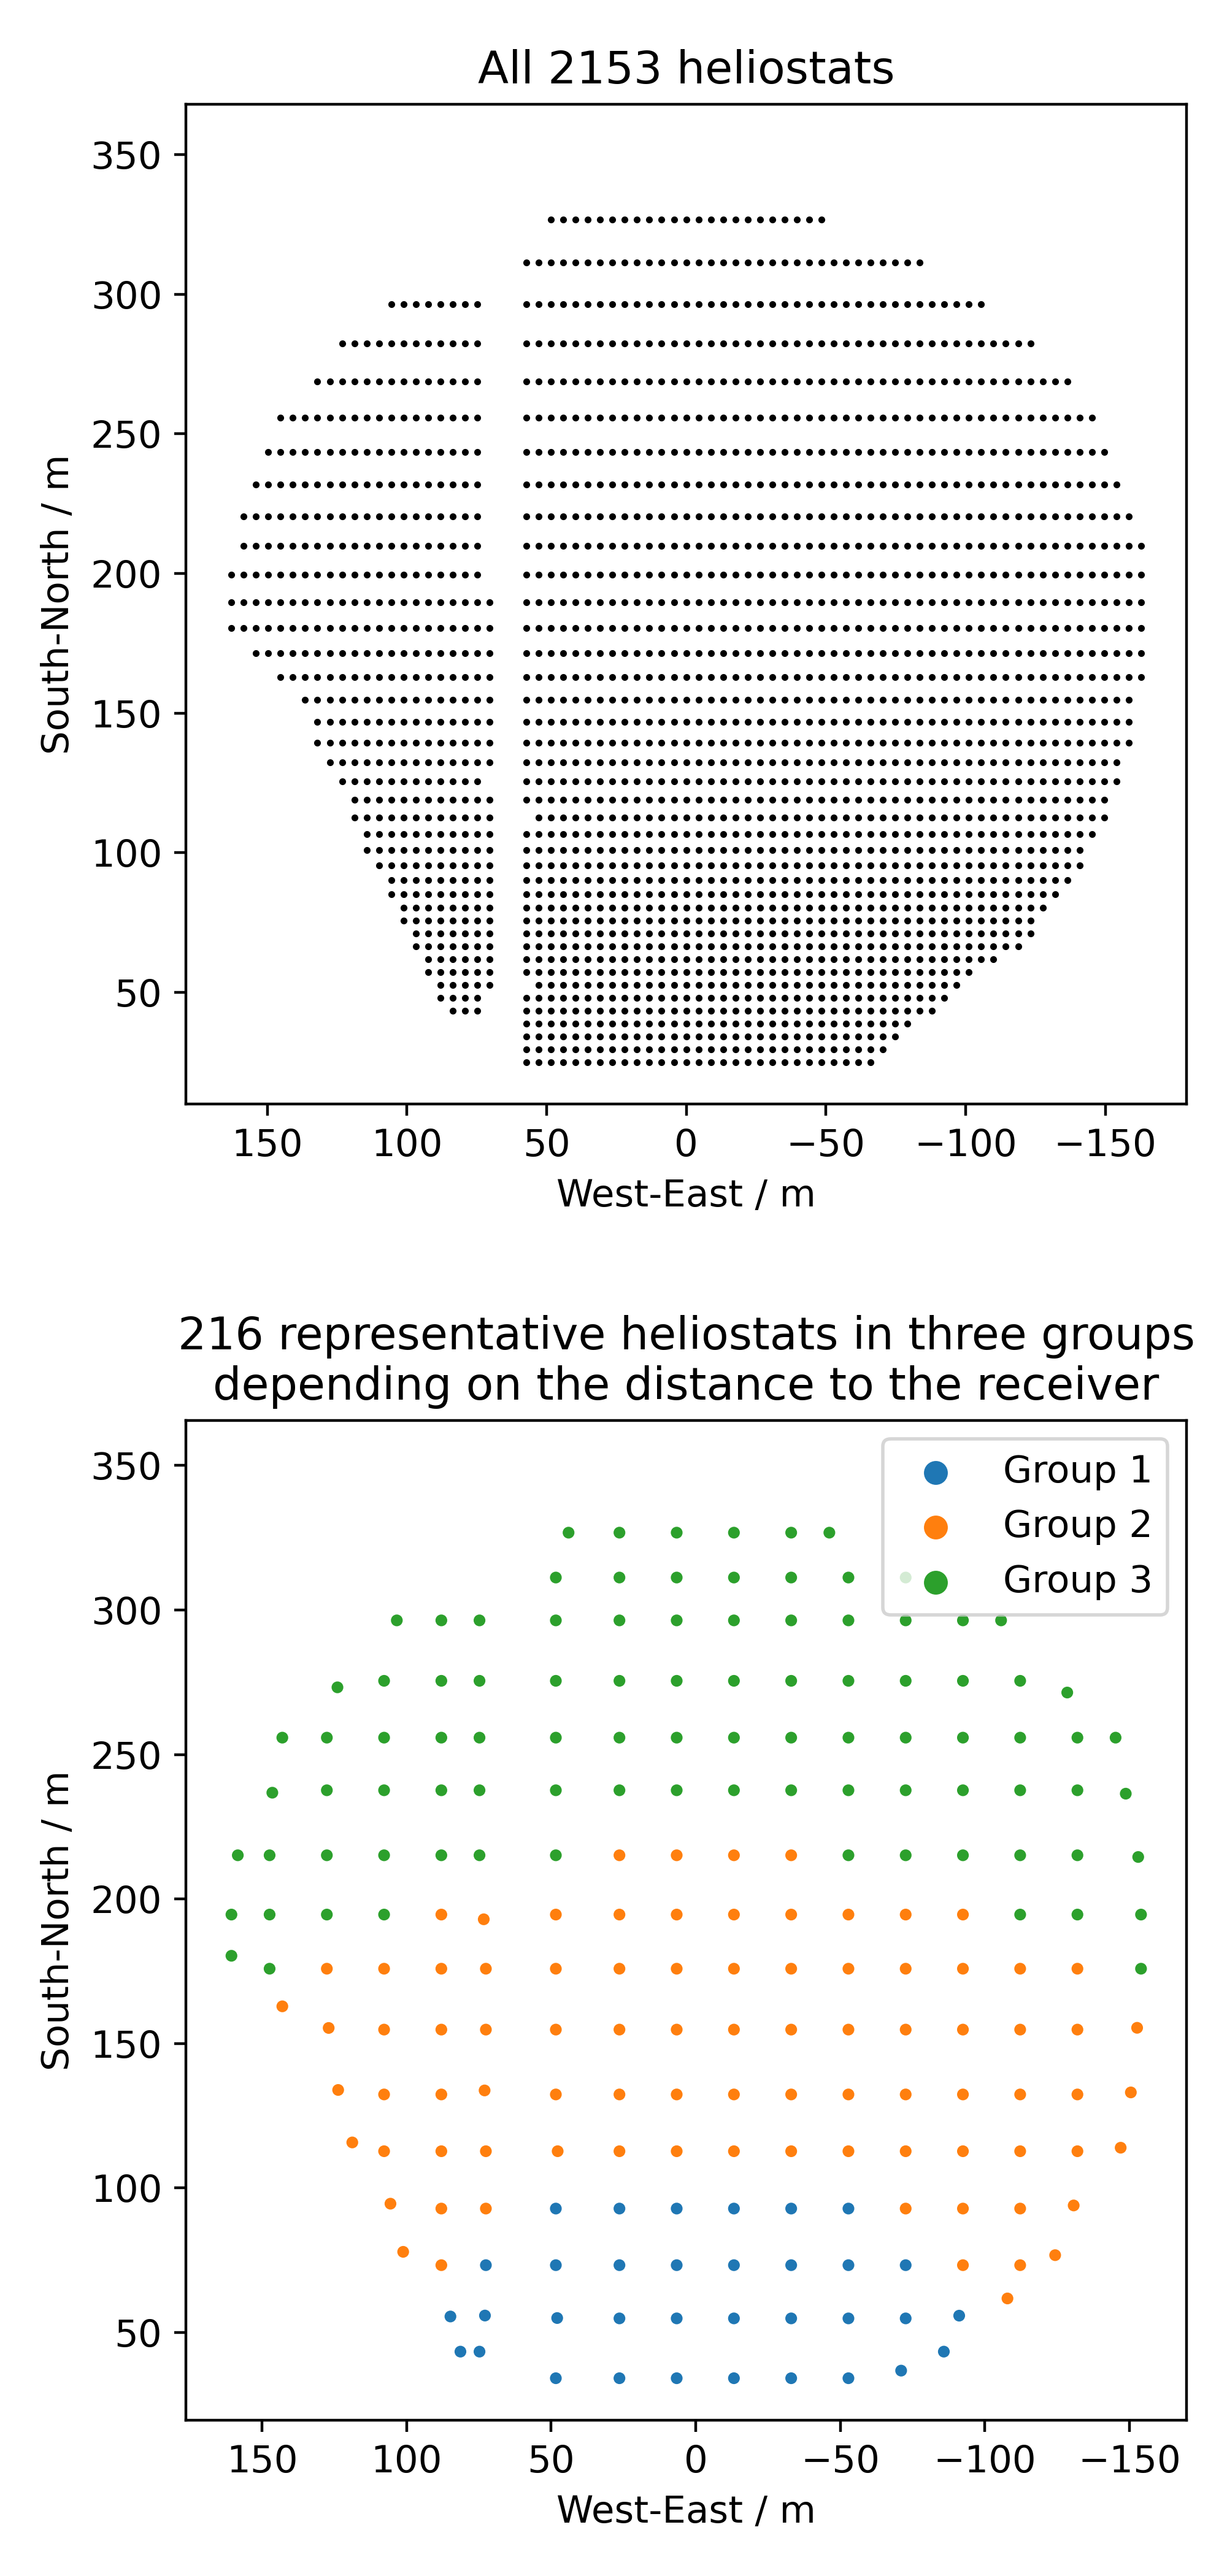
\includegraphics[height=0.7\textheight]{C:/Users/gesc_ma/VSCode MPC Projekt/dynaovrcontroller/dynaovrcontroller/aimpoint_control_scenarios/plots/11_analysis_optical_model/heliostat_field_analysis.png}}
\caption[Gruppierung der Heliostaten am Standort Jülich. Oben ist das vollständige Heliostatenfeld zu sehen, unten die repräsentativen Heliostaten eines $\SI{20}{\metre} \times \SI{20}{\metre}$ Bereiches inklusive Einteilung in drei Gruppen nach Receiverabstand.]{Gruppierung der Heliostaten am Standort Jülich. Oben ist das vollständige Heliostatenfeld zu sehen, unten die repräsentativen Heliostaten eines $\SI{20}{\metre} \times \SI{20}{\metre}$ Bereiches inklusive Einteilung in drei Gruppen nach Receiverabstand.}
    \label{fig_HeliostatenfeldGruppen}
\end{figure}

In dieser Arbeit wird aufgrund des geringen Einflusses auf die Betrachtung der Eingangsgröße $y_{\mathrm{Cent}}$ verzichtet, sodass lediglich ein \textit{dispersion factor} $\kappa$ als Stellgröße jeder der drei Gruppen betrachtet wird.
Gemäß Kapitel \ref{subsubsec_Gruppenverhalten} berechnet sich in Abhängigkeit dieses Faktors ein individueller Zielpunkt jedes Heliostaten auf dem Receiver.

In \cite{Garcia2} wird neben dem finalen Zielpunkt der Heliostaten auch die maximal erlaubte Geschwindigkeit der Nachführung beachtet, sodass jede Zielpunktposition neben dem Streuungsfaktor auch von der jeweils vorigen Positionierung des Heliostaten abhängig ist.
Nachfolgend wird diese Dynamik vernachlässigt.
Es wird stattdessen angenommen, dass die Heliostaten sich innerhalb der Abtastzeit zu einem statischen Zustand unabhängig von der vorigen Position des Zielpunktes bewegen können.
Dies ist in der Parametrisierung des Reglers zu berücksichtigen (vgl. Kapitel \ref{subsubsec_sampletime}).

Durch diese quasistatische Betrachtung des optischen Modells ergibt sich die Möglichkeit, die Heliostatenpositionen in Abhängigkeit des Streuungsfaktors linear zu approximieren.
Auf diese Weise entsteht eine differenzierbare Funktion zur Beschreibung der Zielpunktpositionen.
Weiterhin wird so die komplexe Berechnungsvorschrift nach García (vgl. Abbildung \ref{fig_GarciaAlg}) während der Optimierung vermieden.

Die Güte dieser Approximation zeigt Abbildung \ref{fig_GüteApprox} für die exemplarischen Faktoren $\kappa_1 = 12$, $\kappa_2 = 40$ und $\kappa_3 = 3$, welche so gewählt sind, dass die drei Heliostatengruppen und deren Zielpunktverteilung ersichtlich wird.
Links sind die Zielpunkte der $216$ repräsentativen Heliostaten nach García zu sehen, während mittig die approximierten Zielpunkte dargestellt sind.
Auf der rechten Seite ist für jeden Zielpunkt der Unterschied zwischen diesen Berechnungen zu erkennen, also wie stark jeder approximierte Zielpunkt von seiner durch die ausführliche Berechnungsvorschrift ermittelten Position abweicht.
Die Wurzel des mittleren Quadrates der Abweichung liegt bei $\SI{14}{\centi\metre}$.
Dies ist für die qualitative Betrachtung der Zielpunkte ausreichend, da durch die Brennflecke der Heliostaten nicht nur einzelne Absorbercups erhitzt werden; die Einstrahlungsleistung verteilt sich stattdessen auf den umliegenden Receiverbereich.

\begin{figure}[h!]
    \centering
    \setlength{\fboxsep}{1pt}
    \setlength{\fboxrule}{1pt}
    \fbox{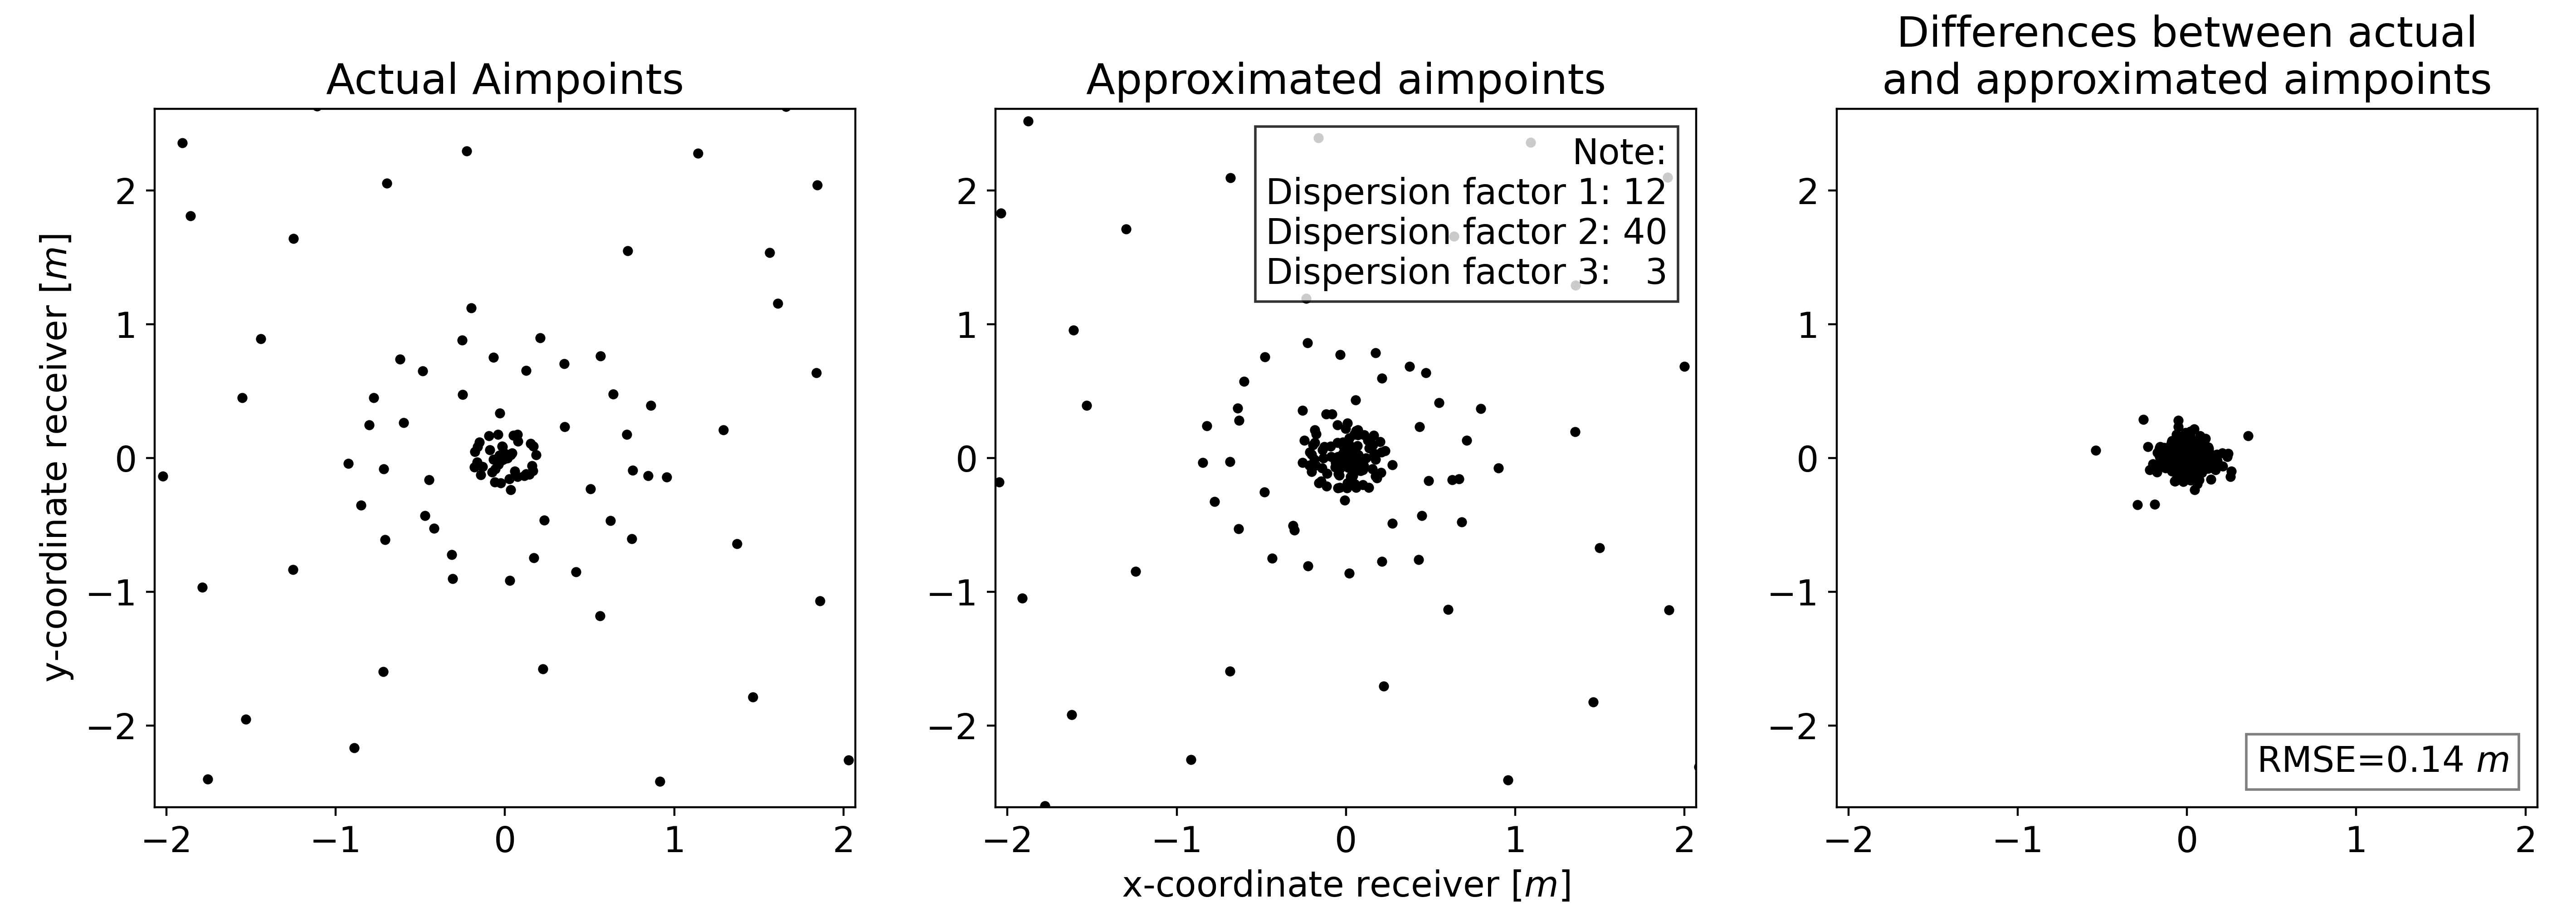
\includegraphics[width=0.98\textwidth]{C:/Users/gesc_ma/VSCode MPC Projekt/dynaovrcontroller/dynaovrcontroller/aimpoint_control_scenarios/plots/11_analysis_optical_model/aimpoint_analysis.png}}
    \caption[Darstellung der Zielpunktverteilung auf dem Receiver für exemplarische Streuungsfaktoren nach García und gemäß der Approximation, sowie Visualisierung der Unterschiede dieser beiden Berechnungen.]{Darstellung der Zielpunktverteilung auf dem Receiver für exemplarische Streuungsfaktoren nach García (Links) und gemäß der Approximation (Mitte), sowie Visualisierung der Unterschiede dieser beiden Berechnungen (Rechts).}
    \label{fig_GüteApprox}
\end{figure}

\subsection{Bestimmung der Flussdichte auf Basis der Zielpunkte} \label{subsec_VerknüfungZielpunkteEinstrahlung}
Um auf der Grundlage der Zielpunkte die Flussdichteverteilung auf dem Receiver errechnen zu können, wird von jedem repräsentativen Heliostaten ein Brennfleck ermittelt, den dieser auf dem Receiver erzeugt.
Zur Berechnung dieses Brennfleckes werden vorberechnete Strahlungskarten aus dem in \cite[S.53ff]{DissBelhomme} vorgestellten Programm \textit{STRAL} (\textbf{S}olar \textbf{T}ower \textbf{Ra}ytracing \textbf{L}aboratory) verwendet.
Dabei handelt es sich um ein Strahlverfolgungsprogramm, welches Sonnenstrahlen auf dem Weg von der Sonne zum Receiver simuliert.

Das Programm nutzt zur Simulation das reale Heliostatenfeld am Standort Jülich.
Auf Basis des Sonnenstandes, der Zielpunktverteilung und der direkt damit einhergehenden Heliostatenpositionen wird für jeden Heliostaten der Verlauf eintreffender Sonnenstrahlen berechnet.
Optische Verluste (vgl. Kapitel \ref{subsec_OptischeVerluste}), die sich geometrisch bedingt ergeben, werden durch die Strahlungsverfolgung bei der Berechnung des Brennfleckes berücksichtigt.
Dazu zählt der Kosinus-Verlust, die Blockierung/Abschattung und die Streuung.

Zusätzlich können in der Berechnung auch optische Verluste in Folge von Heliostateneigenschaften berücksichtigt werden.
Die Reflexionsverluste werden mit $\SI{8}{\percent}$ angenommen, der Spiegelfehler mit $\SI{2}{\milli\radian}$ und der Nachführfehler mit $\SI{1}{\milli\radian}$.
Auch die atmosphärische Abschwächung wird in Abhängigkeit der Entfernung zwischen Receiver und Heliostaten berücksichtigt.
Für eine normierte solare Einstrahlungsleistung von $\SI{1}{\watt\per\metre\squared}$ wird mittels STRAL für jeden der 2153 Heliostaten die Flussdichteverteilung auf dem Receiver ermittelt.
Dafür wird als Zielpunkt zunächst die Mitte des Receivers angenommen, während die Sonnenposition vom 21.06.2022 um 13 Uhr übernommen wird ($\SI{17.72}{\degree}$ in der Azimuth und $\SI{61.65}{\degree}$ in der Elevationsebene).
Eine Übersicht über die in STRAL berücksichtigten optischen Fehler zeigt Tabelle \ref{tab_optischeVerlustequantität}.

\begingroup
\renewcommand{\arraystretch}{1.2}
\begin{table}[ht!]
    \caption[Übersicht über die quantitative Berücksichtigung der optischen Verluste in der Flussdichteberechnung mit STRAL]{Übersicht über die quantitative Berücksichtigung der optischen Verluste in der Flussdichteberechnung mit STRAL}
    \centering
    \begin{tabular}{m{0.37\textwidth}m{0.56\textwidth}}
        \rowcolor{white}
        \toprule
        Optischer Verlust           & Intensität                                         \\
        \midrule
        Kosinus-Verluste            & In Abhängigkeit der jeweiligen Heliostatenposition \\
        Blockierung/Abschattung     & In Abhängigkeit der jeweiligen Heliostatenposition \\
        Streuung                    & In Abhängigkeit der jeweiligen Heliostatenposition \\
        Reflexivität der Spiegel    & $\SI{8}{\percent}$                                 \\
        Spiegelfehler               & $\SI{2}{\milli\radian}$                            \\
        Nachführfehler              & $\SI{1}{\milli\radian}$                            \\
        Atmosphärische Abschwächung & In Abhängigkeit der jeweiligen Heliostatenposition \\
        \toprule
    \end{tabular}
    \label{tab_optischeVerlustequantität}
\end{table}
\endgroup

Durch Überlagerung aller Flussdichteverteilungen von Heliostaten aus einem $\SI{20}{\metre} \times \SI{20}{\metre}$ Bereich entstehen die Brennflecke der repräsentativen Heliostaten dieses Bereiches.
Wie in Kapitel \ref{sec_Nowcasting} erläutert, ist das Ziel des Nowcastings die Prädiktion der direkten Einstrahlung in dieser Genauigkeit (vgl. Abbildung \ref{fig_EinstrahlungNowcasting}).
Der entsprechende DNI-Wert jedes Bereiches wird anschließend mit der normierten Flussdichteverteilung der repräsentativen Heliostaten multipliziert.
Für einen wolkenfreien Himmel wird eine direkte Einstrahlung von $\SI{850}{\watt\per\metre\squared}$ angenommen.
Abbildung \ref{fig_CasadiFluxmap} zeigt exemplarisch die Flussdichteverteilung des repräsentativen Heliostaten mit dem geringsten Receiverabstand für wolkenlose Bedingungen.

\begin{figure}[h!]
    \centering
    \setlength{\fboxsep}{1pt}
    \setlength{\fboxrule}{1pt}
    \fbox{
        \hfill
        \begin{subfigure}[b]{0.48\textwidth}
            \centering
            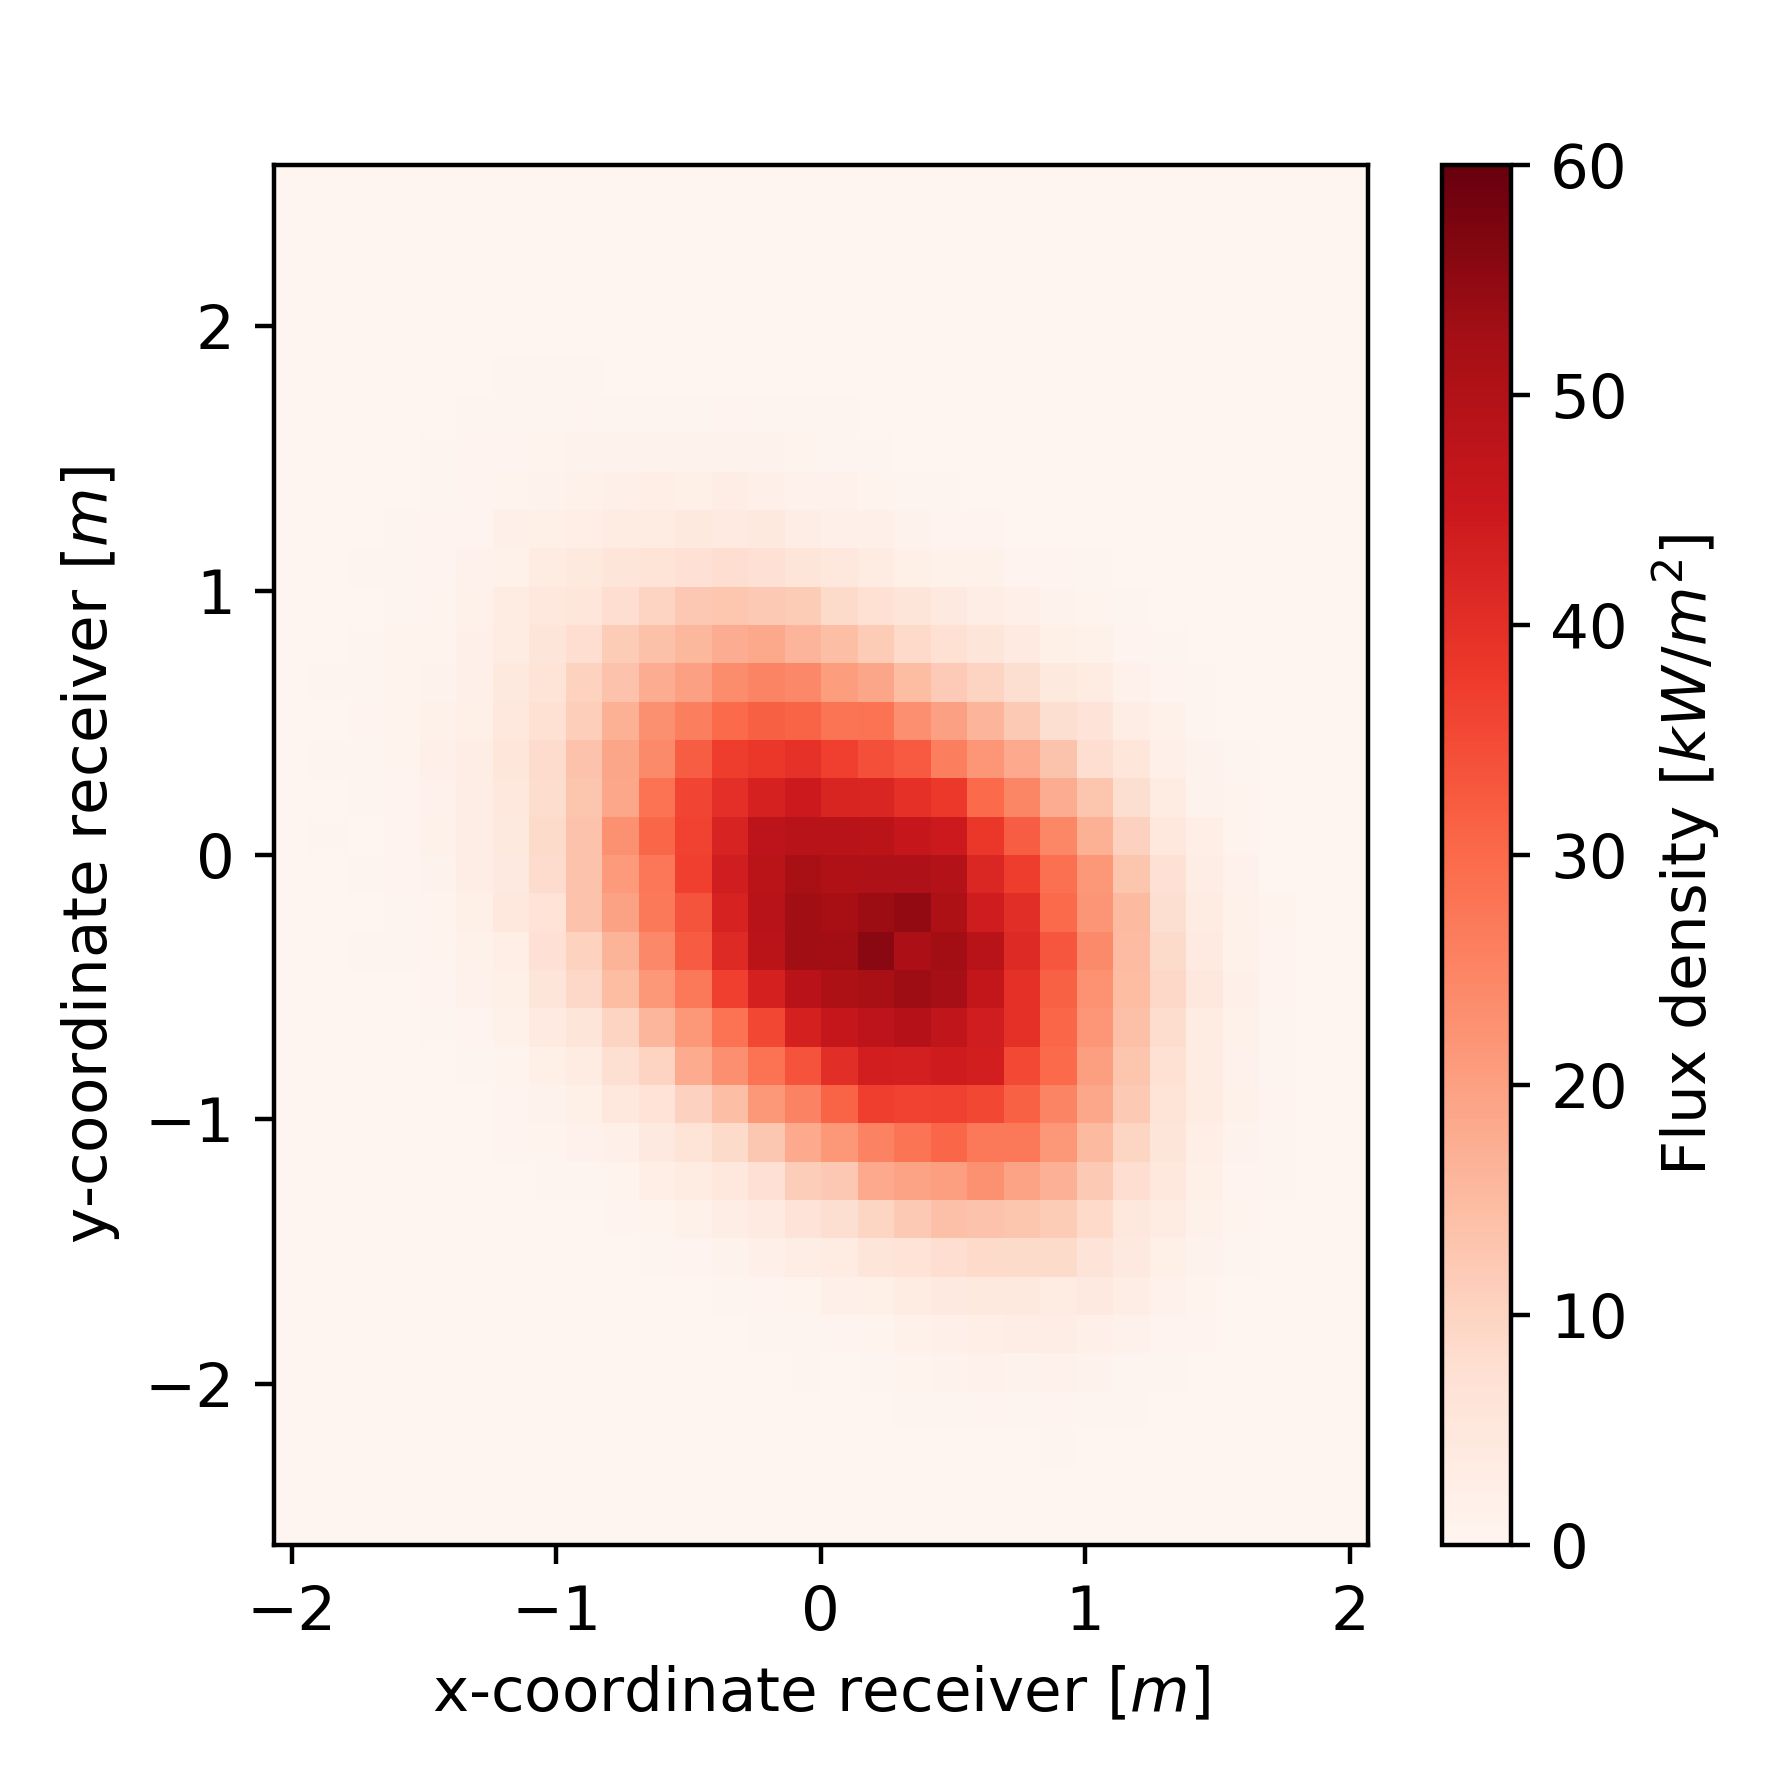
\includegraphics[width=\linewidth]{C:/Users/gesc_ma/VSCode MPC Projekt/dynaovrcontroller/dynaovrcontroller/aimpoint_control_scenarios/plots/11_analysis_optical_model/2D visualization of casadi fluxmap interpolant.png}
            \label{fig_CasadiFluxmap2D}
        \end{subfigure}
        \hfill
        \begin{subfigure}[b]{0.48\textwidth}
            \centering
            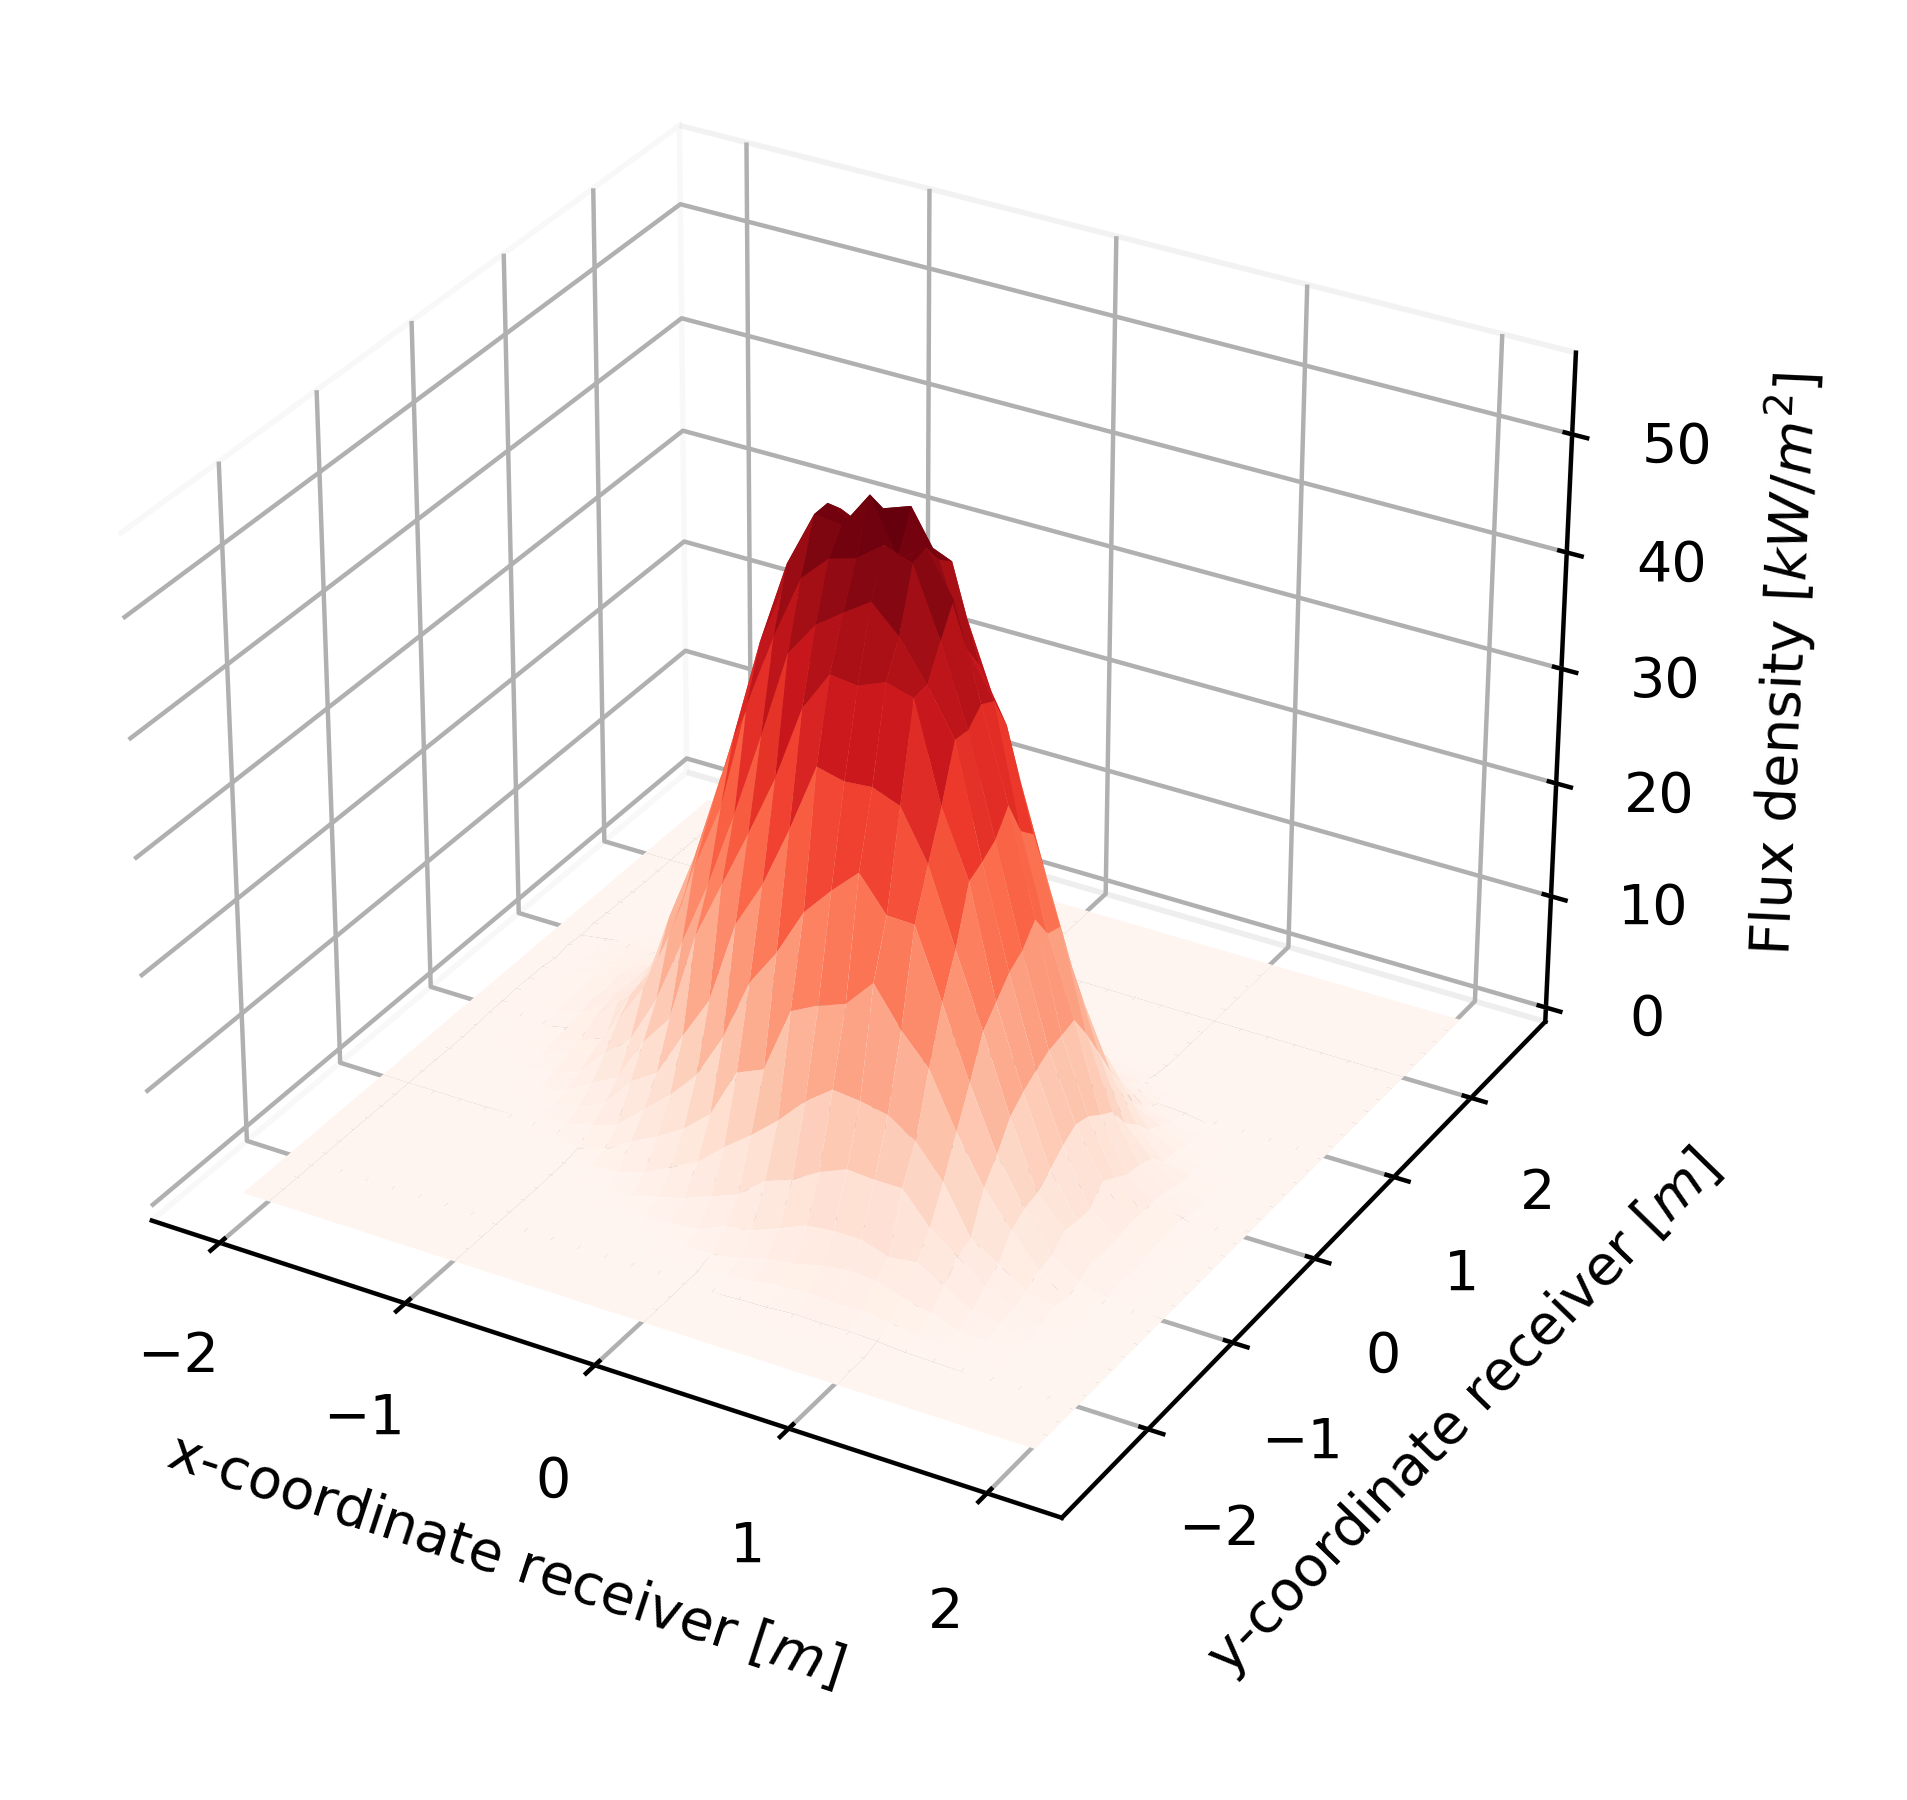
\includegraphics[width=\linewidth]{C:/Users/gesc_ma/VSCode MPC Projekt/dynaovrcontroller/dynaovrcontroller/aimpoint_control_scenarios/plots/11_analysis_optical_model/3D visualization of casadi fluxmap interpolant.png}
            \label{fig_CasadiFluxmap3D}
        \end{subfigure}
        \hfill}
    \caption[Exemplarische Flussdichteverteilung des repräsentativen Heliostaten mit dem geringsten Abstand zum Receiver in 2D und 3D]{Exemplarische Flussdichteverteilung des repräsentativen Heliostaten mit dem geringsten Abstand zum Receiver in 2D (Links) und 3D (Rechts)}
    \label{fig_CasadiFluxmap}
\end{figure}

Es ist erkennbar, dass für jeden der $1080$ Cups ein diskreter Wert der Flussdichte vorliegt.
Durch Überlagerung der Flussdichteverteilungen aller repräsentativer Heliostaten wird die gesamte Flussdichte auf dem Receiver bestimmt.
Wie in Kapitel \ref{sec_optischesModell} erwähnt, dient das bis hier vorgestellte optische Modell der Simulation, da es auf den exakten Strahlungskarten basiert.

Im Gegensatz dazu werden die Einstrahlungskarten für das optische Teilmodell zur Optimierung durch 2D-Gauss-Verteilungen approximiert.
Dies verringert den Rechenaufwand auf Kosten der Genauigkeit.
Abbildung \ref{fig_GaussFluxmap} zeigt die approximierte Flussdichteverteilung für den receivernächsten repräsentativen Heliostaten.
Der durchschnittliche RMSE aller 216 Flussdichteapproximationen beträgt $\SI{0.33}{\kilo\watt\per\metre\squared}$.

\begin{figure}[h!]
    \centering
    \setlength{\fboxsep}{1pt}
    \setlength{\fboxrule}{1pt}
    \fbox{
        \hfill
        \begin{subfigure}[b]{0.48\textwidth}
            \centering
            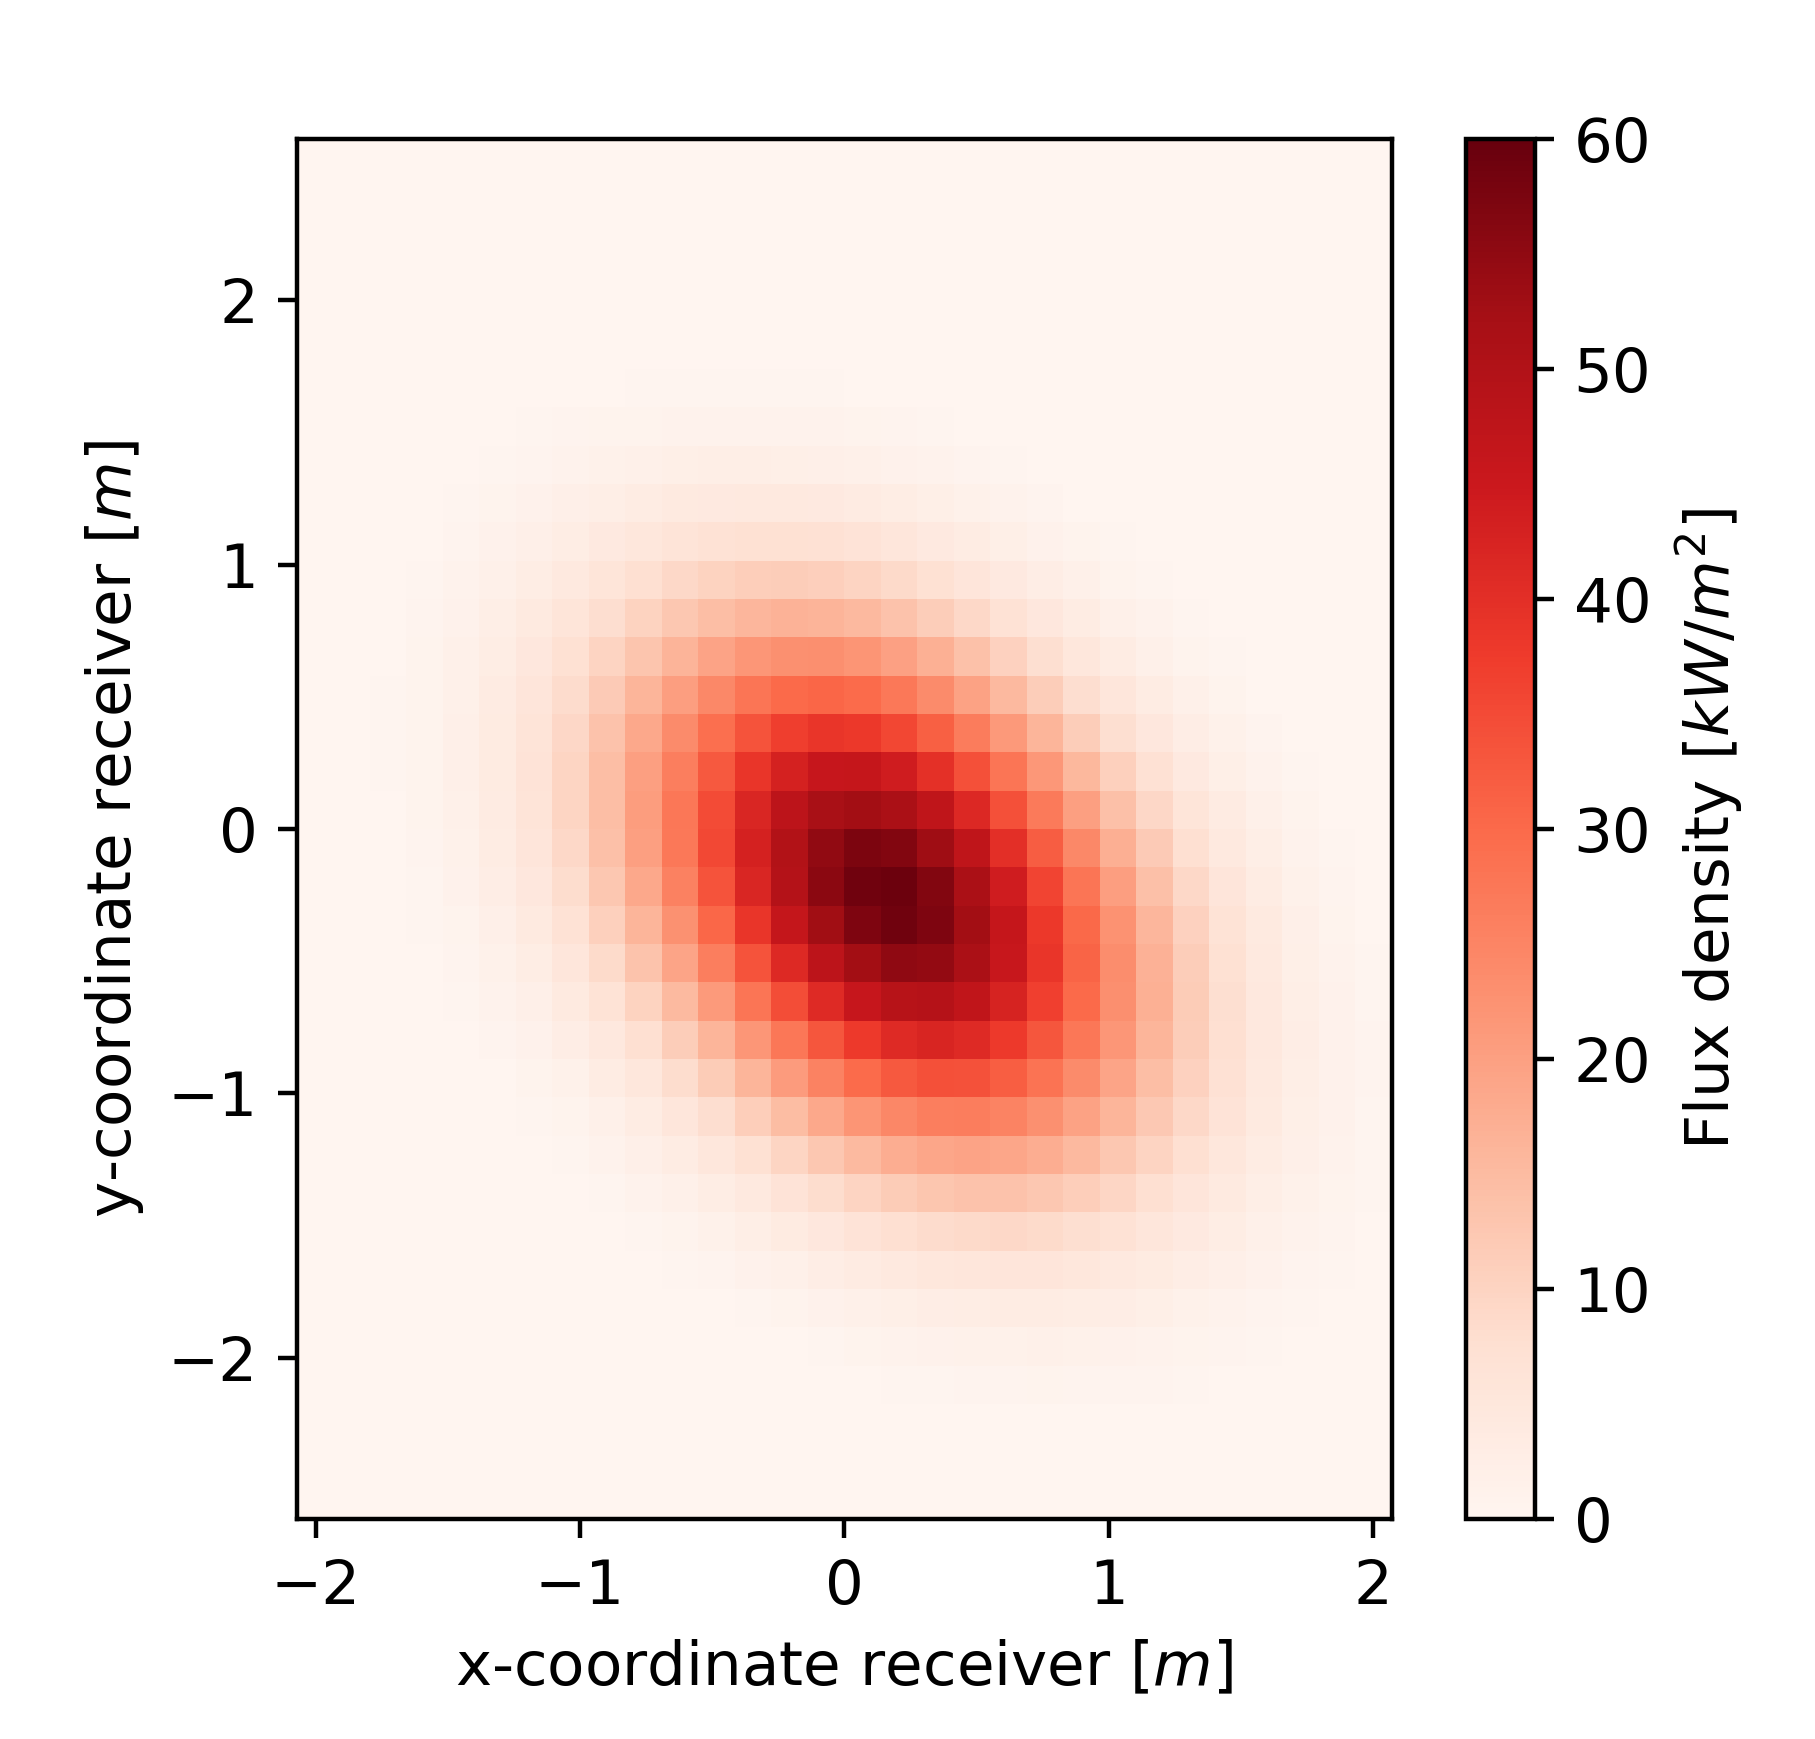
\includegraphics[width=\linewidth]{C:/Users/gesc_ma/VSCode MPC Projekt/dynaovrcontroller/dynaovrcontroller/aimpoint_control_scenarios/plots/11_analysis_optical_model/2D visualization of gaussian fluxmap interpolant.png}
            \label{fig_GaussFluxmap2D}
        \end{subfigure}
        \hfill
        \begin{subfigure}[b]{0.48\textwidth}
            \centering
            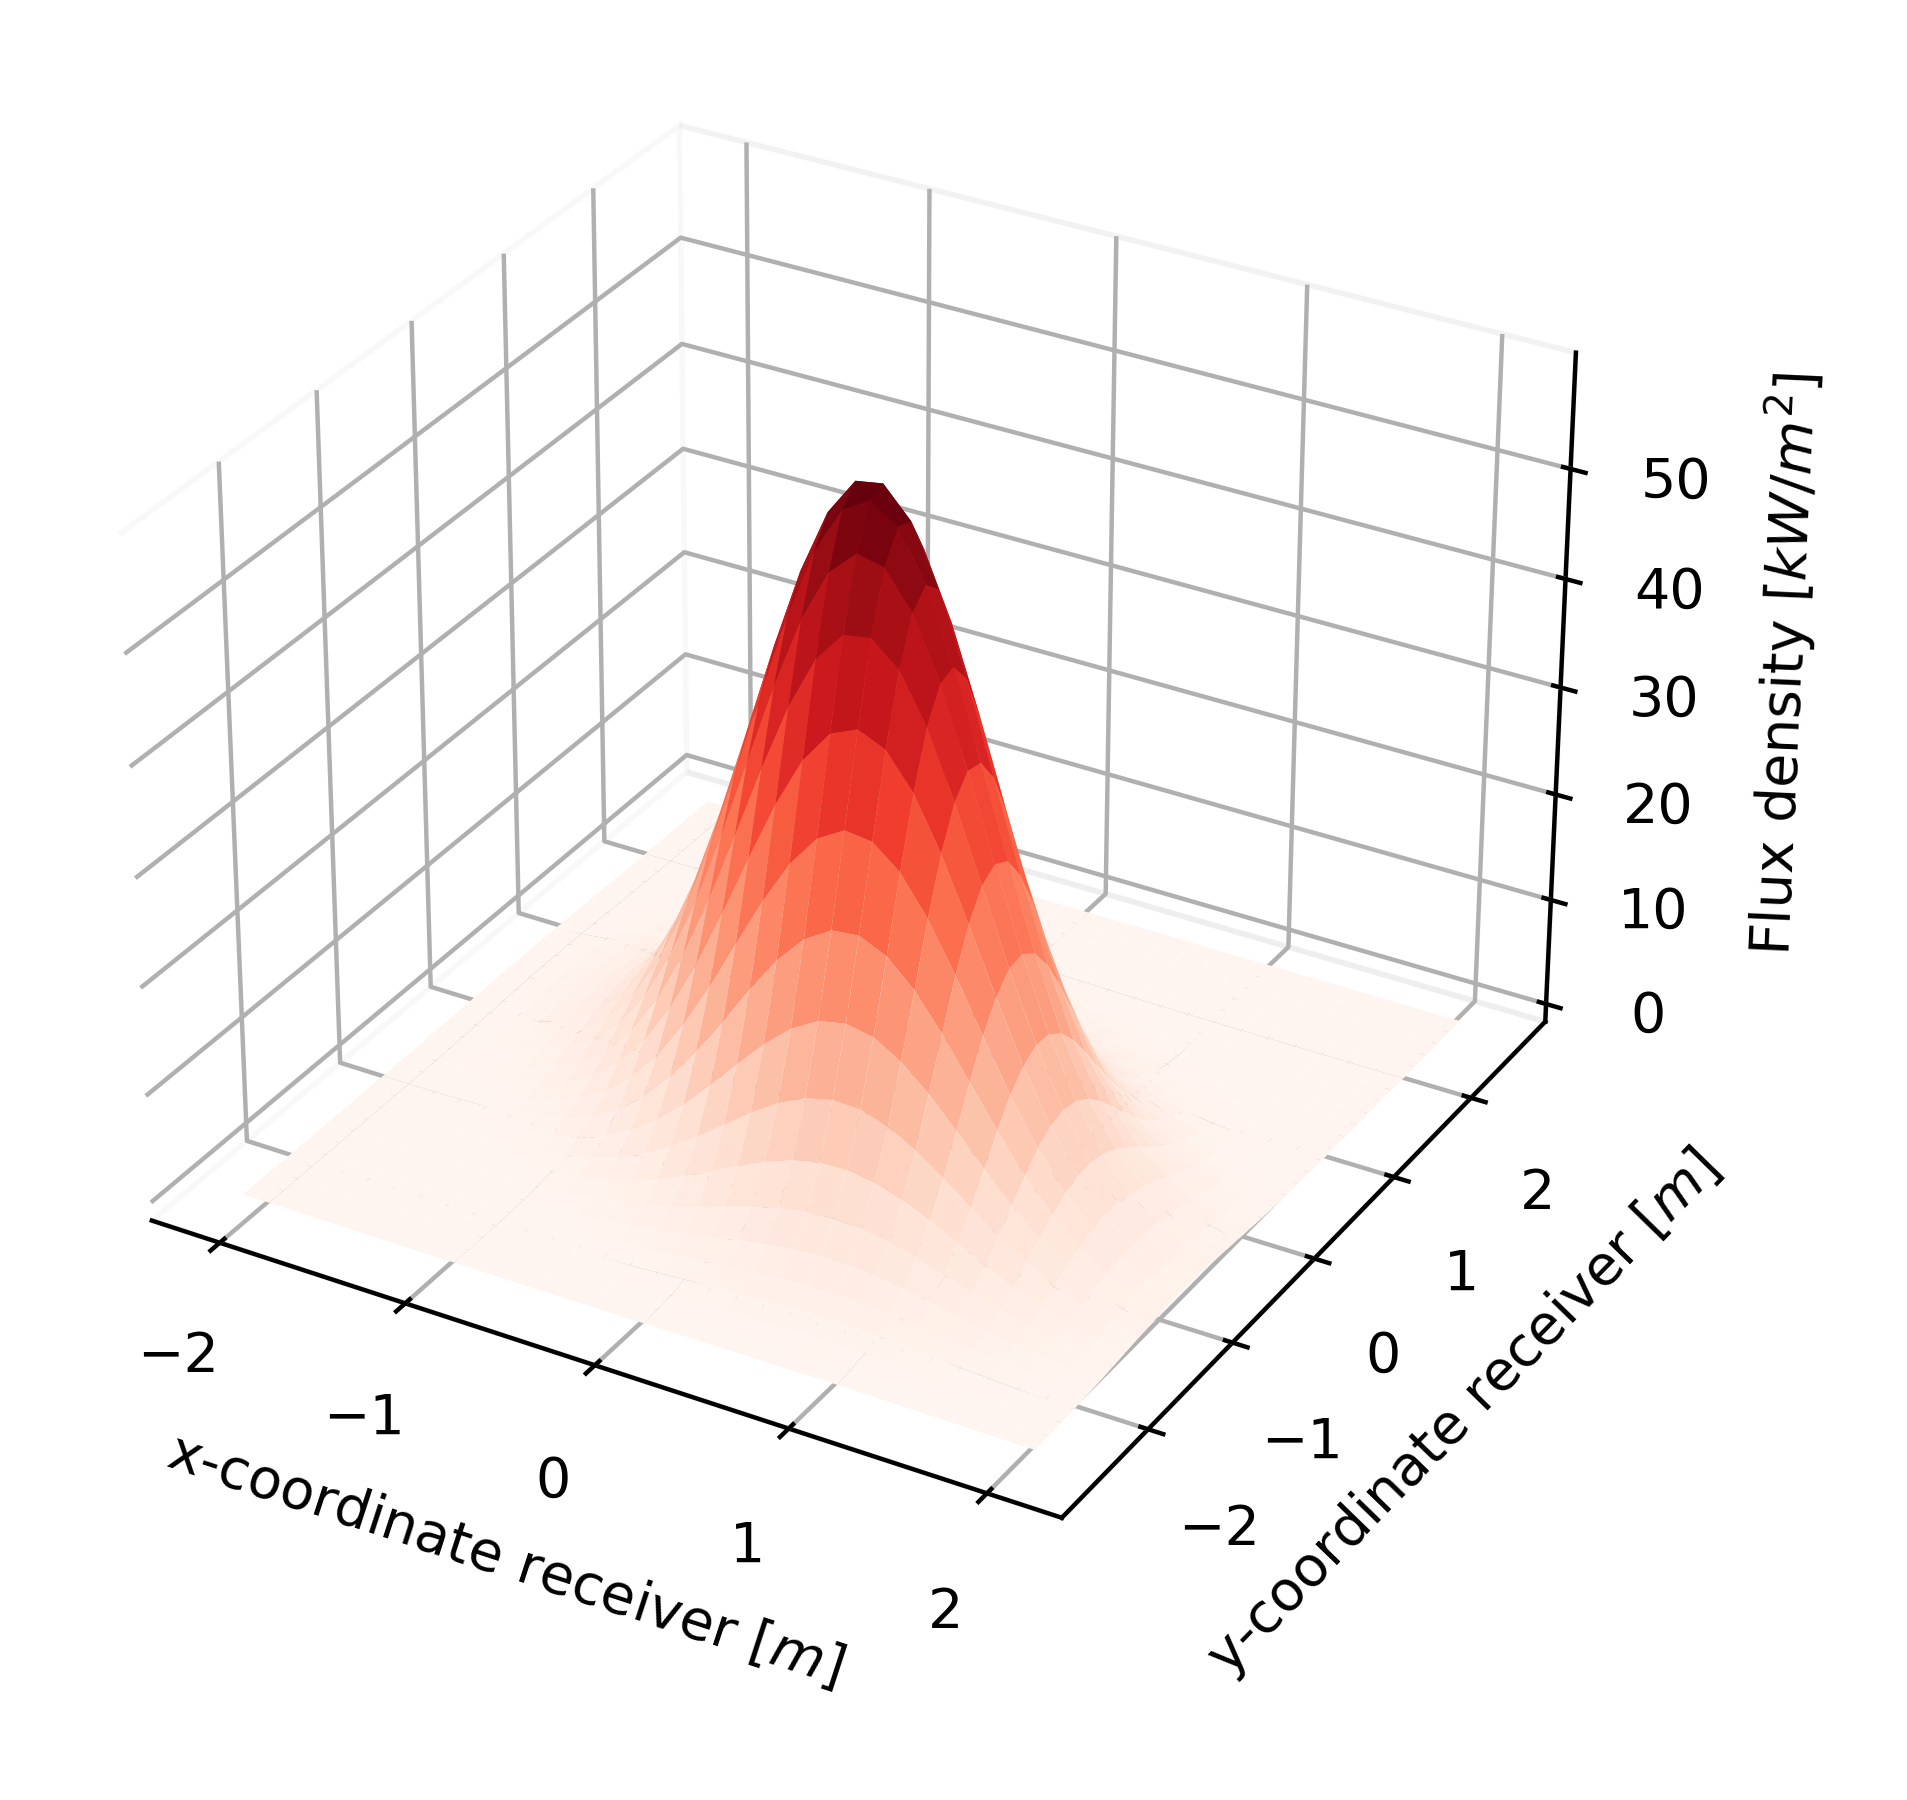
\includegraphics[width=\linewidth]{C:/Users/gesc_ma/VSCode MPC Projekt/dynaovrcontroller/dynaovrcontroller/aimpoint_control_scenarios/plots/11_analysis_optical_model/3D visualization of gaussian fluxmap interpolant.png}
            \label{fig_GaussFluxmap3D}
        \end{subfigure}
        \hfill}
    \caption[Exemplarische approximierte Flussdichteverteilung des repräsentativen Heliostaten mit dem geringsten Abstand zum Receiver in 2D und 3D]{Exemplarische approximierte Flussdichteverteilung des repräsentativen Heliostaten mit dem geringsten Abstand zum Receiver in 2D (Links) und 3D (Rechts)}
    \label{fig_GaussFluxmap}
\end{figure}

\pagebreak
\section{Kopplung der Teilmodelle} \label{sec_KopplungModelle}
Der Solarturm in Jülich besteht aus $\SI{36}{} \times \SI{30}{}$ Absorbercups.
Jeder dieser $1080$ Cups wird wie in Kapitel \ref{subsec_ModellCup} erläutert durch zwei Differentialgleichungen und zwei algebraische Gleichungen beschrieben.
Aufgrund des daraus resultierenden hohen Rechenaufwandes zur Lösung eines Optimierungsproblems dieser Größe wird das Modell auf $\SI{6}{} \times \SI{5}{}$ Cups reduziert.

Das thermische Modell wird dabei so angepasst, dass je $36$ Blendendurchmesser der Absorbercups gemittelt werden, um den Massenstrom durch einen repräsentativen Cup des jeweiligen Receiverbereiches zu erhalten.
Dabei stimmt der maximale Luftmassenstrom des $\SI{36}{} \times \SI{30}{}$ Cup Systems mit dem des diskretisierten Systems überein.
Auf diese Weise wird gewährleistet, dass der identische Enthalpiestrom in das System aufgenommen werden kann und die identische Flussdichteverteilung auch dieselbe Fronttemperatur des Receivers zur Folge hat.
Der zulässige Bereich des Massenstroms und des Einstellwertes (vgl. Abschnitt \ref{subsec_BeschreibungLüftungsDyn}) werden entsprechend dieser Diskretisierung angepasst.
Insgesamt ergibt sich so ein System aus $30$ repräsentativen Cups.
Dieses kann unter Berücksichtigung der Lüftungsdynamik durch $60+2$ Differentialgleichungen und $60$ algebraischen Gleichungen beschrieben werden.

Die gemeinsame Größe des optischen und des thermischen Teilmodells ist die Flussdichte auf den Absorbercups.
Durch die Reduzierung des thermischen Modells auf $30$ Cups muss auch das optische Modell entsprechend angepasst werden.
Abbildung \ref{fig_statischerZielpunkt363065} zeigt die Diskretisierung des optischen Simulationsmodells exemplarisch, für den Fall, dass alle Zielpunkte auf den Mittelpunkt des Receivers eingestellt sind. \pagebreak

\begin{figure}[h!]
    \centering
    \setlength{\fboxsep}{1pt}
    \setlength{\fboxrule}{1pt}
    \fbox{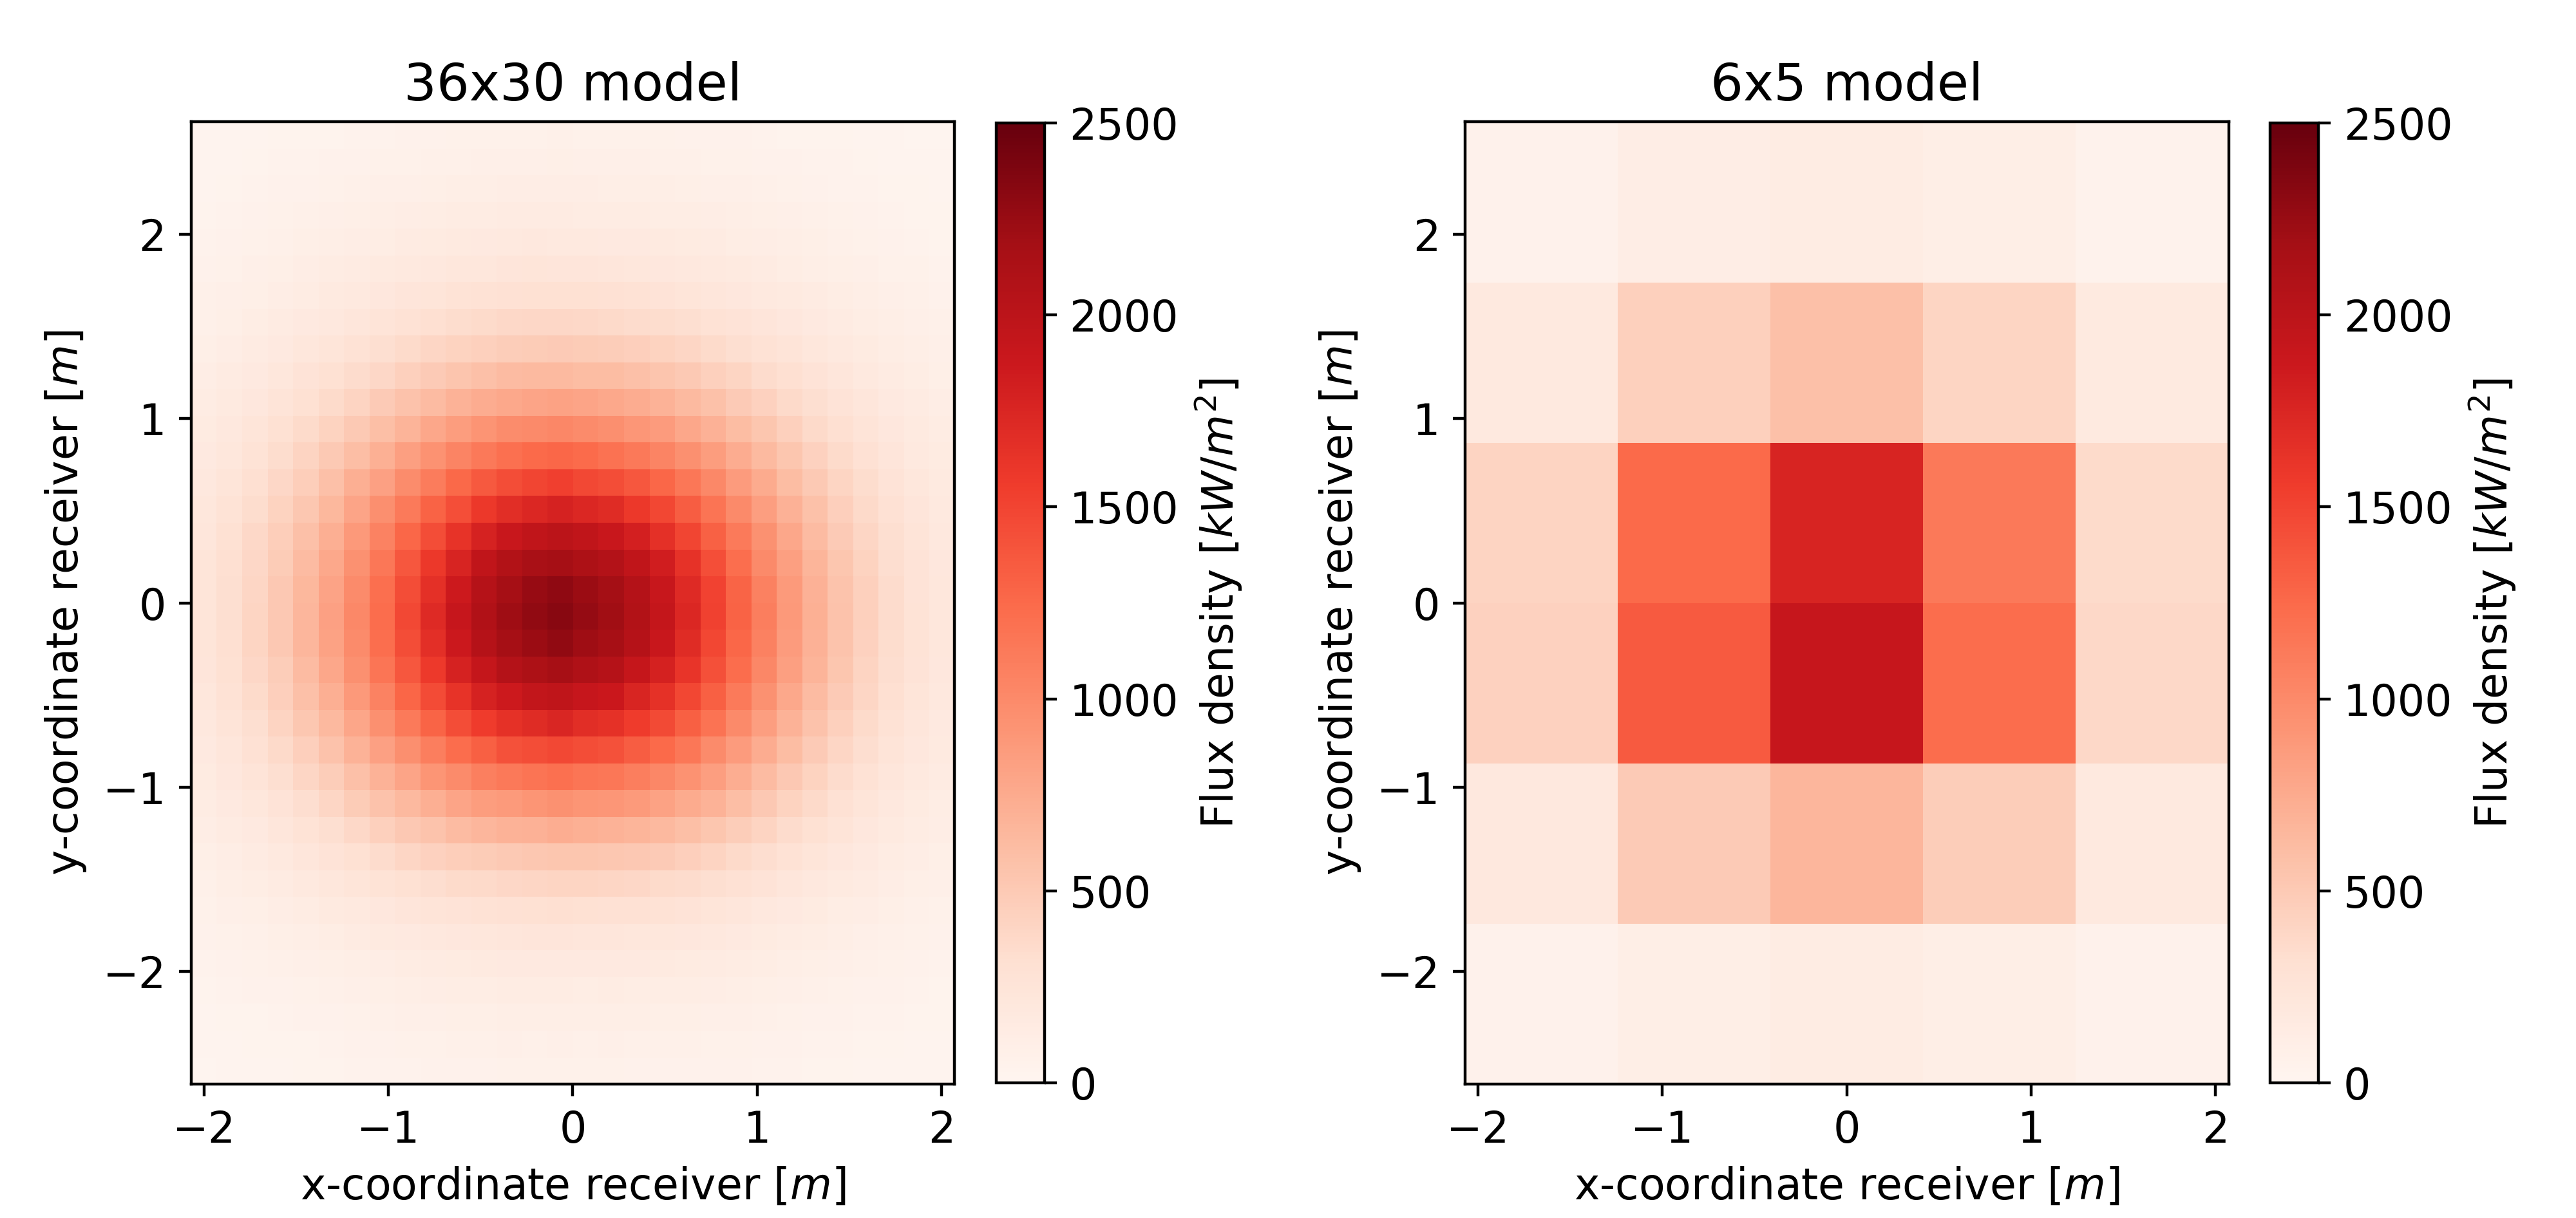
\includegraphics[width=0.93\textwidth]{C:/Users/gesc_ma/VSCode MPC Projekt/dynaovrcontroller/dynaovrcontroller/aimpoint_control_scenarios/plots/11_analysis_optical_model/model_discretization.png}}
    \caption[Überlagerung der Flussdichteverteilungen aller repräsentativer Heliostaten des simulativen optischen Modells am Receivermittelpunkt für das Modell mit 1080 Cups und das vereinfachte Modell mit 30 Cups]{Überlagerung der Flussdichteverteilungen aller repräsentativer Heliostaten des simulativen optischen Modells am Receivermittelpunkt für das Modell mit 1080 Cups (Links) und das vereinfachte Modell mit 30 Cups (Rechts)}
    \label{fig_statischerZielpunkt363065}
\end{figure}

Aus dem Optimierungsproblem zur Leistungsoptimierung des Receivers (Gleichung \ref{eq_OptimierungZielpunkteDiskret}) folgt, dass jeder der betrachten Cups möglichst nah an der maximal zulässigen Temperatur betrieben wird.
Dementsprechend sind im Realbetrieb nicht alle Heliostaten in die Mitte ausgerichtet, sodass eine homogenere Flussdichteverteilung auf dem Receiver entsteht und der Einfluss dieser Diskretisierung weniger signifikant ist, als aufgrund von Abbildung \ref{fig_statischerZielpunkt363065} anzunehmen ist.
Für die drei Faktoren $\kappa_1 = 25$, $\kappa_2 = 42$ und $\kappa_3 = 12$ ergibt sich für das simulative optische Modell beispielhaft die in Abbildung \ref{fig_dispersionSTRAL36300605} erkennbare Flussdichteverteilung.

\enlargethispage{\baselineskip}
\begin{figure}[h!]
    \centering
    \setlength{\fboxsep}{1pt}
    \setlength{\fboxrule}{1pt}
    \fbox{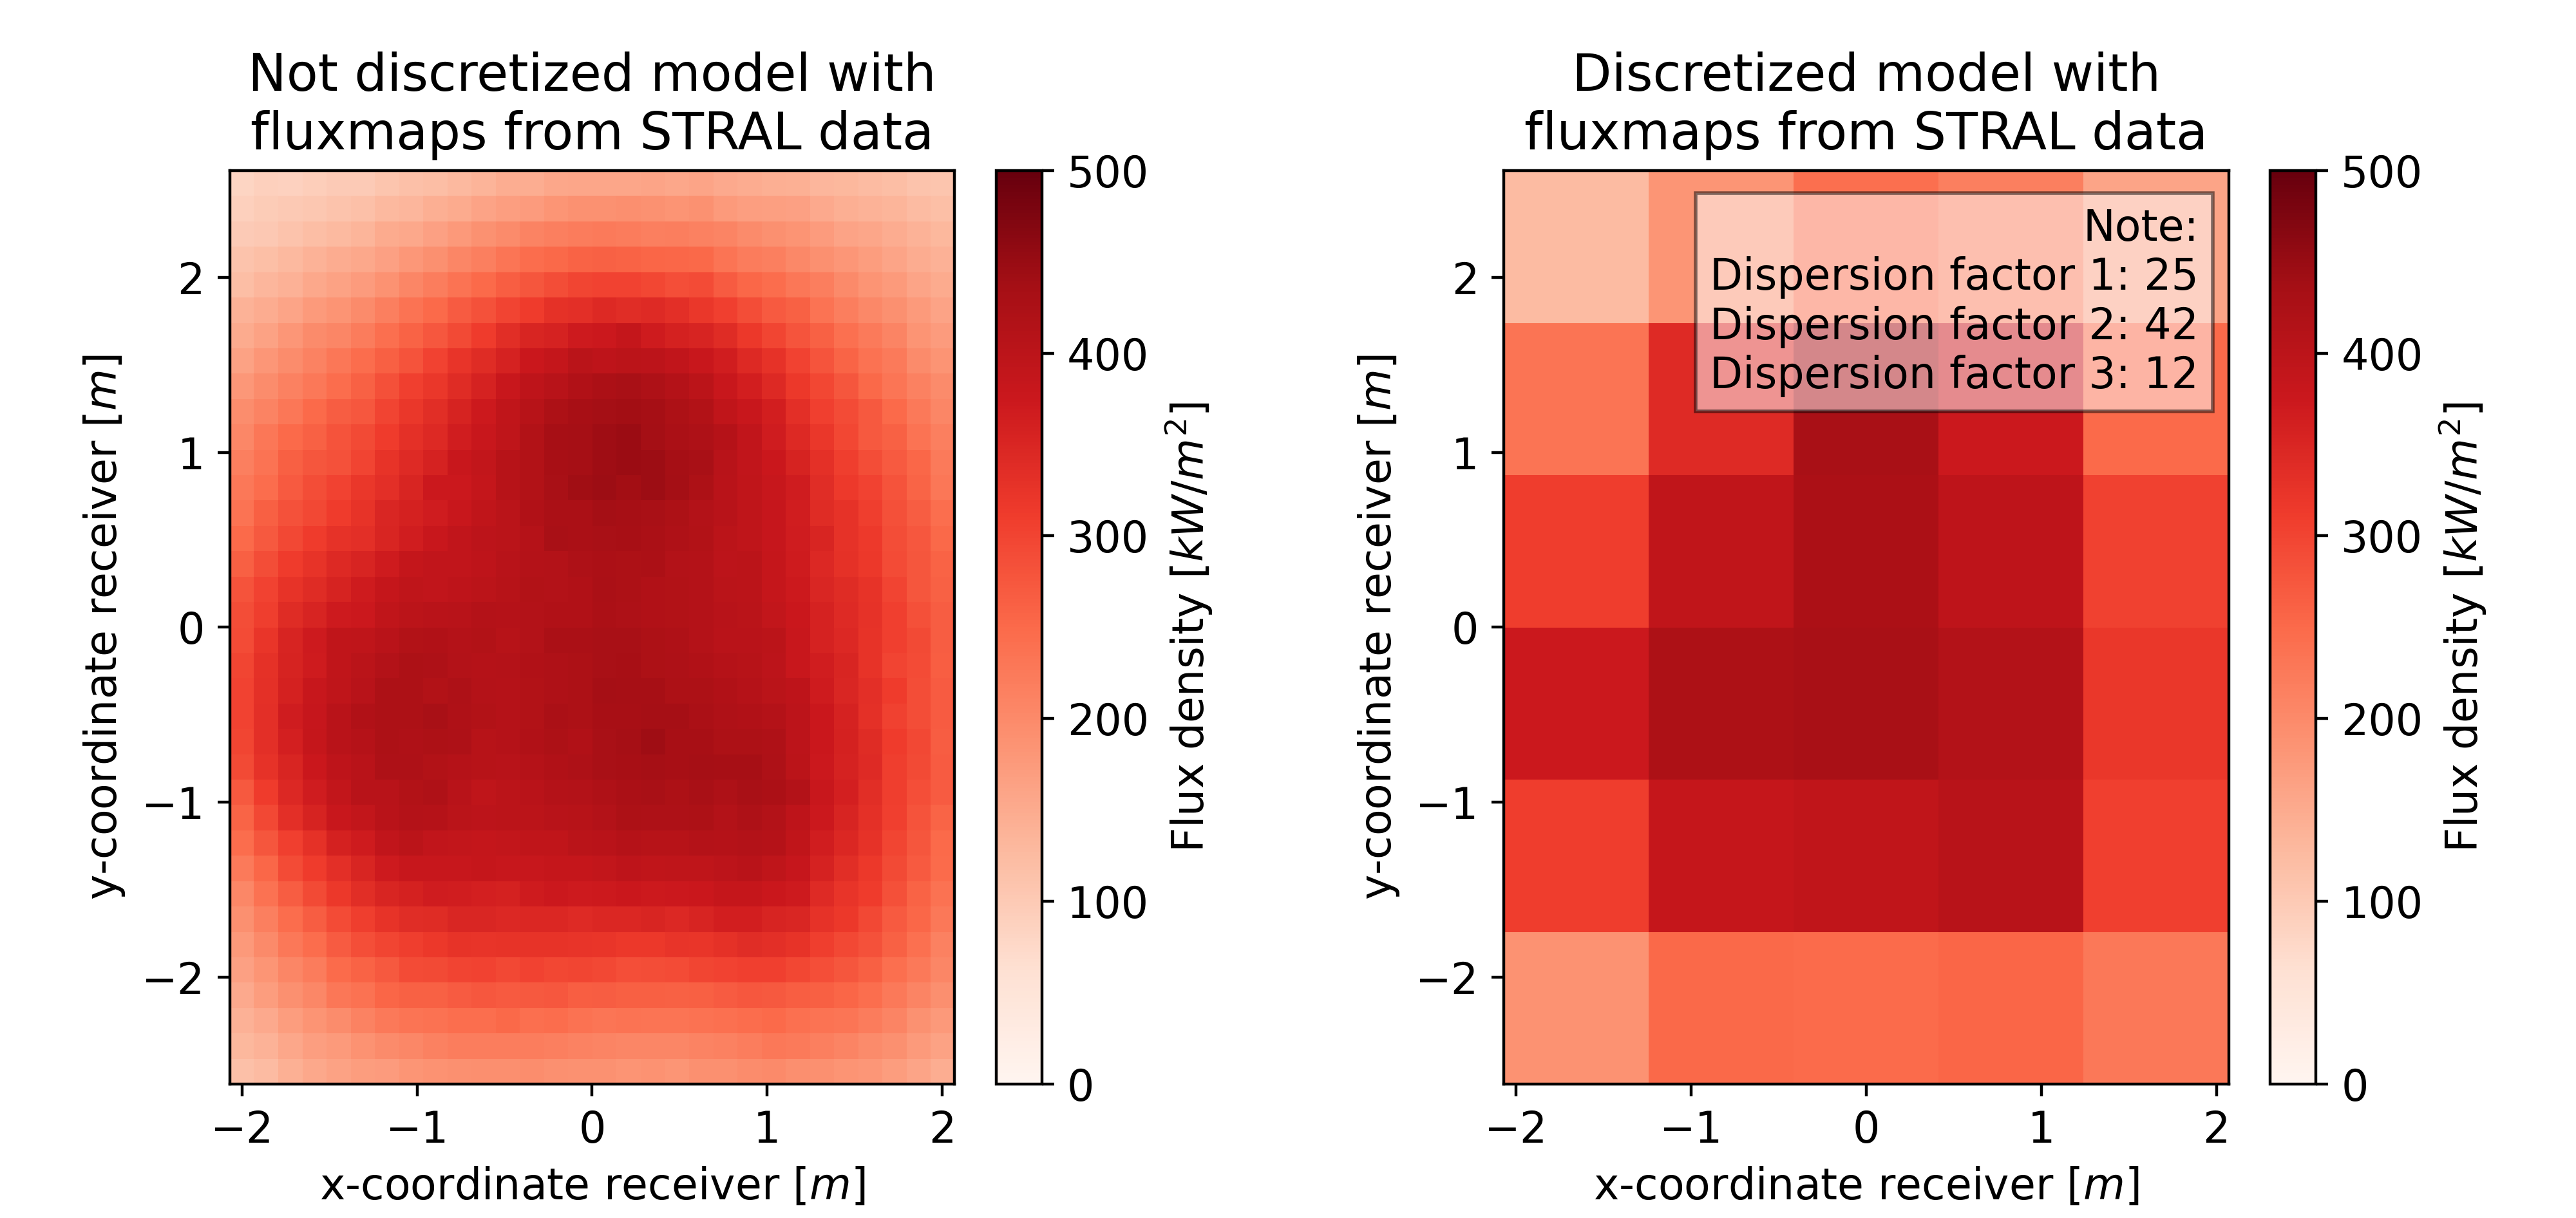
\includegraphics[width=0.93\textwidth]{C:/Users/gesc_ma/VSCode MPC Projekt/dynaovrcontroller/dynaovrcontroller/aimpoint_control_scenarios/plots/11_analysis_optical_model/discretization_differences_dispersion_distribution_casadi.png}}
    \caption[Homogenere Flussdichteverteilung im vollständigen Modell und im vereinfachten Modell]{Homogenere Flussdichteverteilung im vollständigen Modell (Links) und im vereinfachten Modell (Rechts)}
    \label{fig_dispersionSTRAL36300605}
\end{figure}

Die Unterschiede zwischen dem optischen Modell zur Simulation auf Basis der Flussdichtekarten nach STRAL und dem optischen Modell zur Optimierung ist in Abbildung \ref{fig_UnterschiedoptischeModelle} zu sehen.
Diese zeigt links für die ausgewählten Streuungsfaktoren die Flussdichteverteilung gemäß der STRAL Daten sowie rechts die der approximierten Daten.
Es ist erkennbar, dass die Approximation nur geringfügige Flussdichteunterschiede mit einem RMSE von $\SI{14.4}{\kilo\watt\per\metre\squared}$ verursacht.


\begin{figure}[h!]
    \centering
    \setlength{\fboxsep}{1pt}
    \setlength{\fboxrule}{1pt}
    \fbox{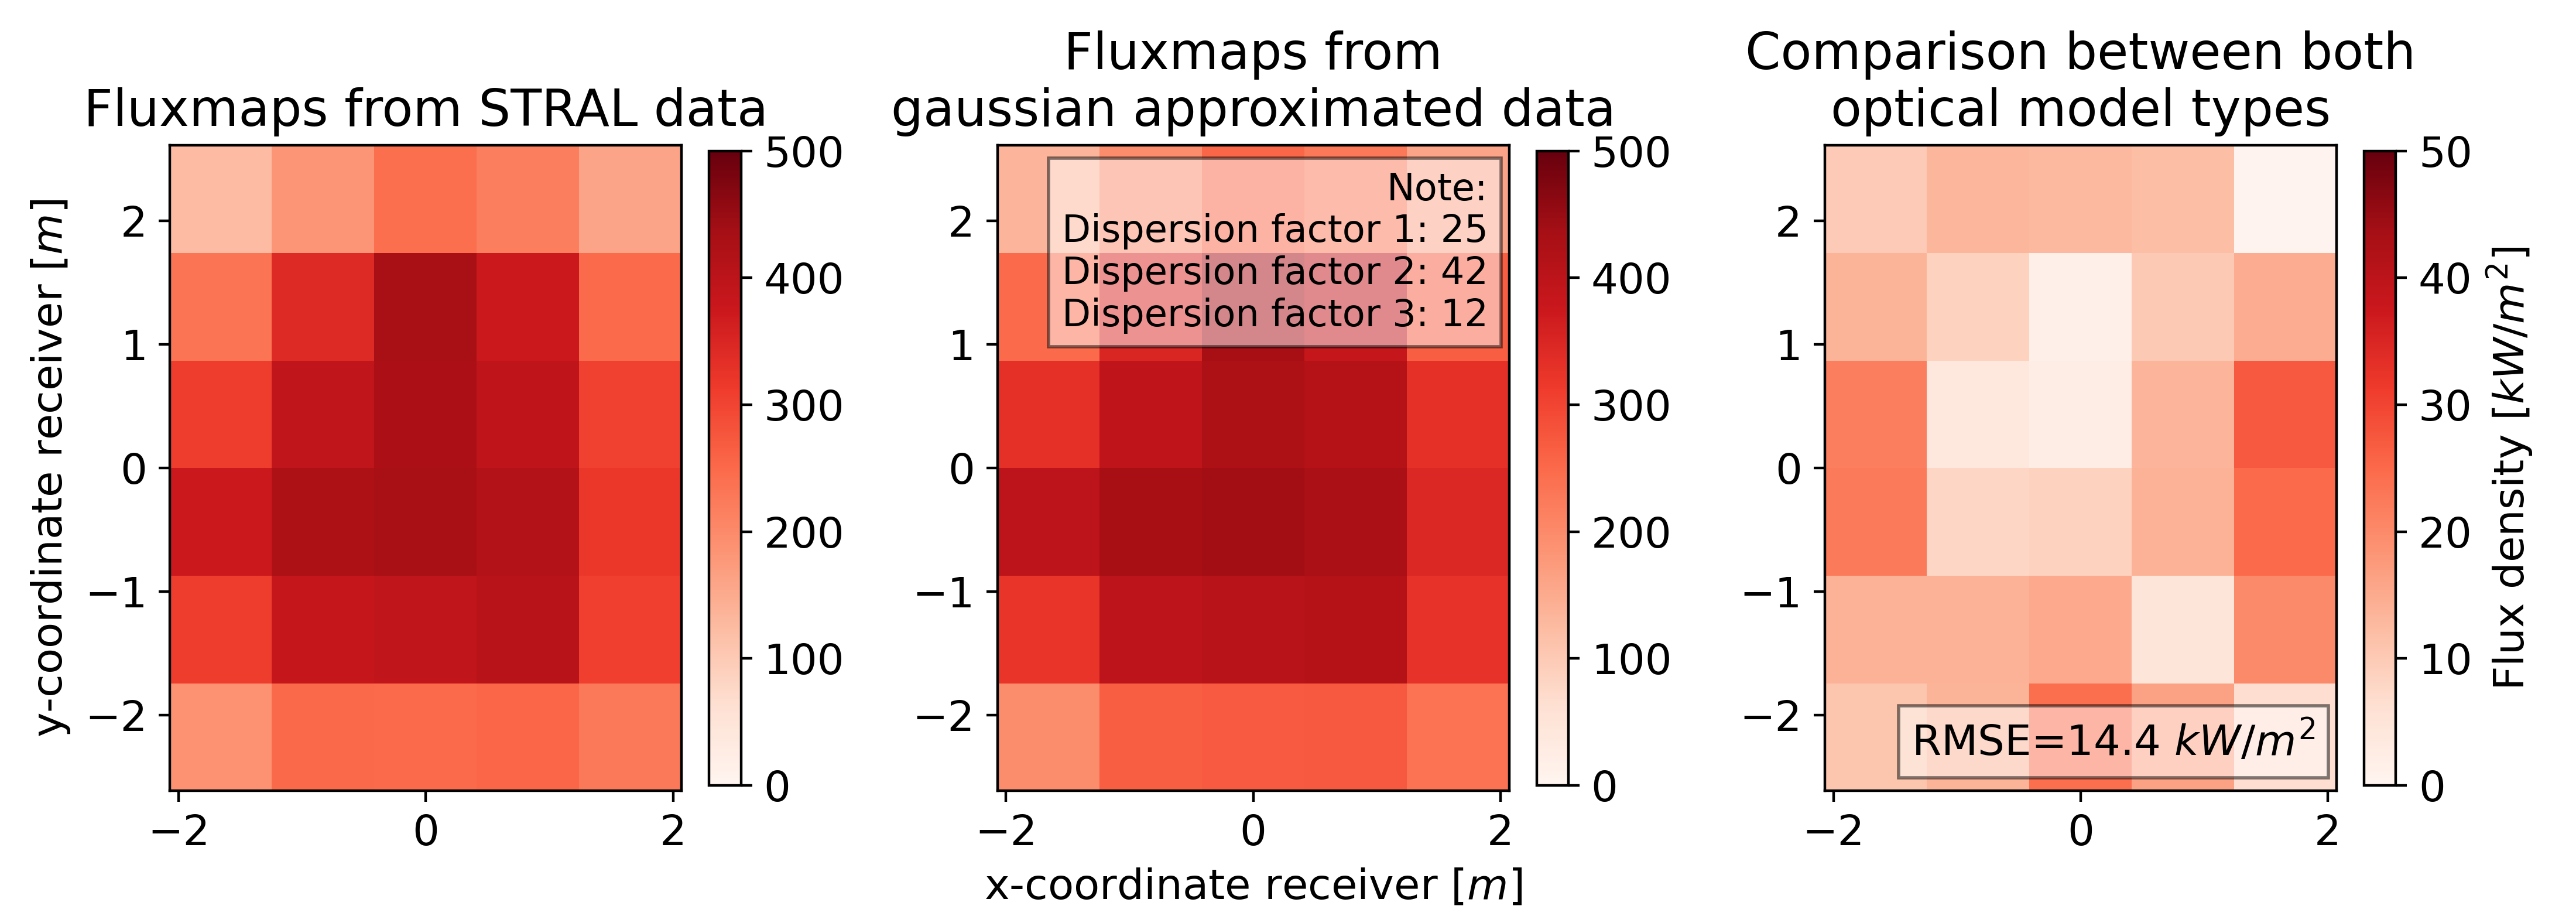
\includegraphics[width=0.98\textwidth]{C:/Users/gesc_ma/VSCode MPC Projekt/dynaovrcontroller/dynaovrcontroller/aimpoint_control_scenarios/plots/11_analysis_optical_model/interpolant_differences.png}}
    \caption[Visualisierung der Unterschiede der optischen Teilmodelle für eine beispielhafte Zielpunktverteilung]{Visualisierung der Unterschiede der optischen Teilmodelle für eine beispielhafte Zielpunktverteilung}
    \label{fig_UnterschiedoptischeModelle}
\end{figure}

Abbildung \ref{fig_RMSEüberdispersion} visualisiert den Betrag des RMSE für einen variablen Wert von $\kappa_1$, wobei zu sehen ist, dass für die gewählten Streuungsfaktoren von $\kappa_2 = 42$ und $\kappa_3 = 12$ ein maximaler RMSE von $\SI{20.0}{\kilo\watt\per\metre\squared}$ für $\kappa_1 = 2$ auftritt.

\begin{figure}[h!]
    \centering
    \setlength{\fboxsep}{1pt}
    \setlength{\fboxrule}{1pt}
    \fbox{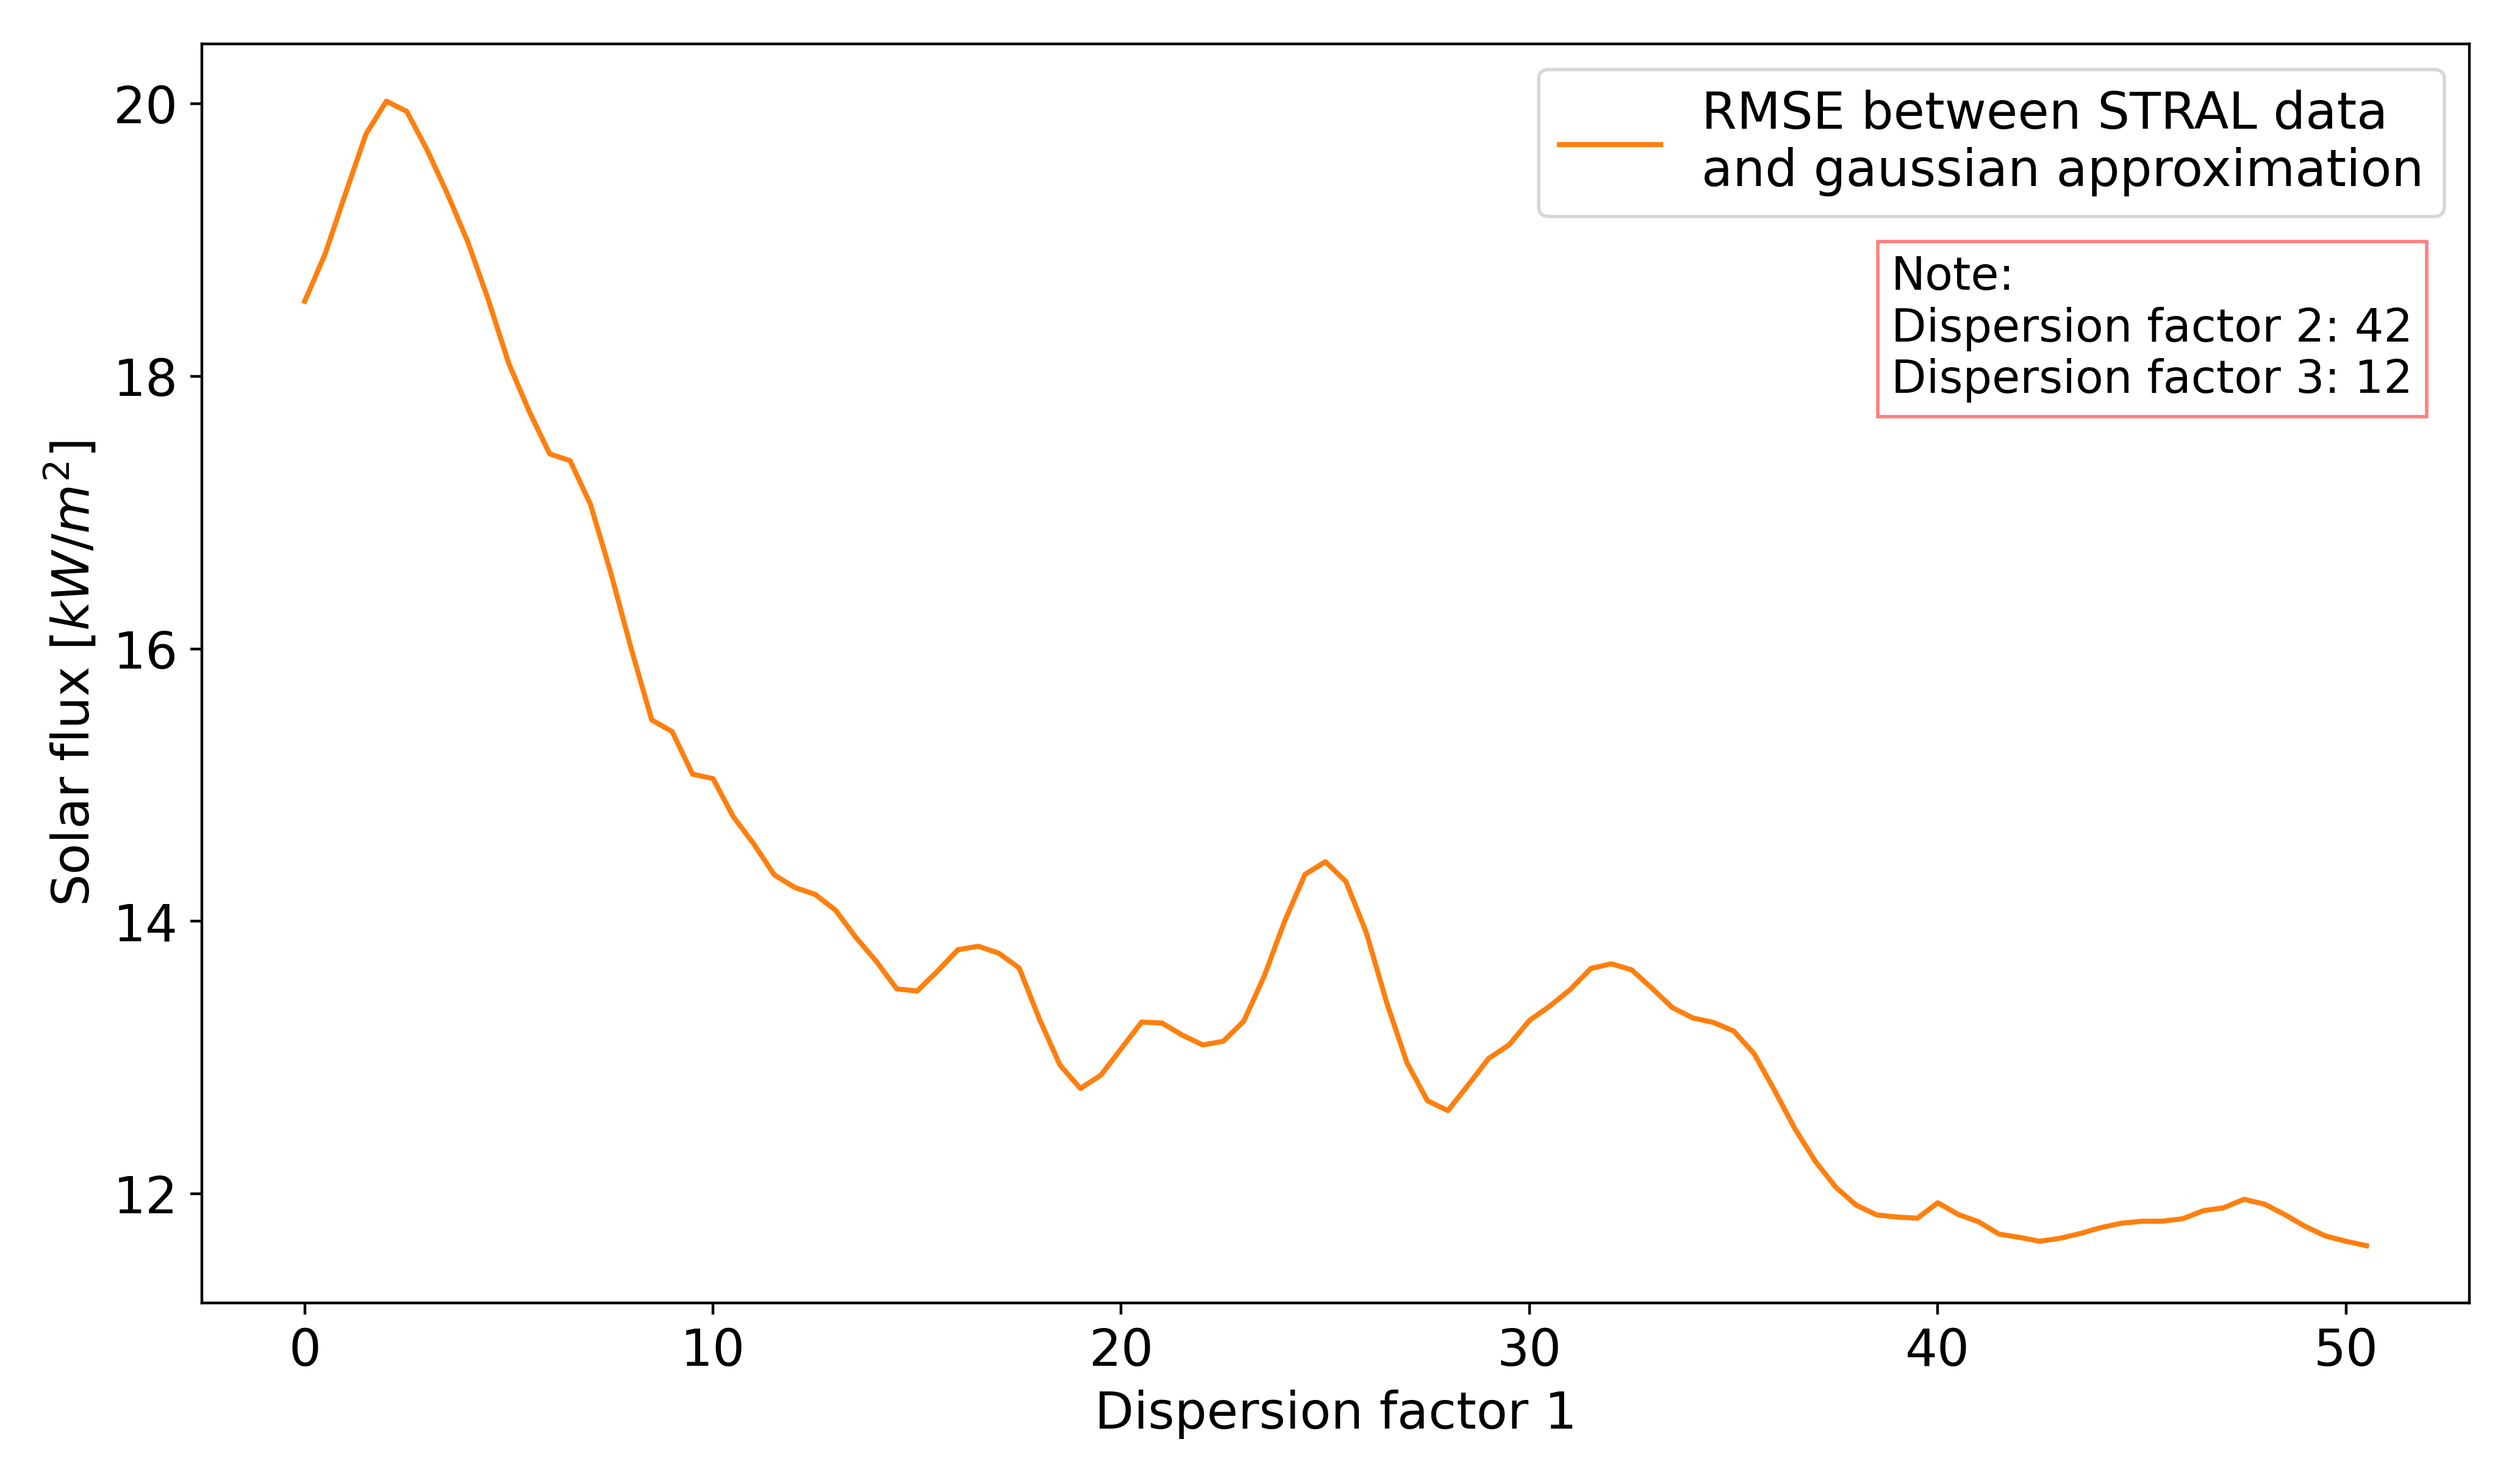
\includegraphics[width=0.98\textwidth]{C:/Users/gesc_ma/VSCode MPC Projekt/dynaovrcontroller/dynaovrcontroller/aimpoint_control_scenarios/plots/11_analysis_optical_model/maximum_relative_error_over_dis_factor.png}}
\caption[Visualisierung der Unterschiede der optischen Teilmodelle durch den Verlauf des RMSE bei variablem Streuungsfaktor $\kappa_1$]{Visualisierung der Unterschiede der optischen Teilmodelle durch den Verlauf des RMSE bei variablem Streuungsfaktor $\kappa_1$}
    \label{fig_RMSEüberdispersion}
\end{figure}

Beide optischen Teilmodelle resultieren in der Flussdichteverteilung für $30$ Absorbercups.
Somit wird jedem der Cups im thermischen Modell eine individuelle Flussdichte vorgegeben.
Die wesentlichen Schritte der Modellbildung sowie die Kopplung der Teilmodelle sind in Abbildung \ref{fig_ZusammenfassungKopplung} zu sehen.

\begin{figure}[p]
    \centering
    \setlength{\fboxsep}{1pt}
    \setlength{\fboxrule}{1pt}
\rotatebox{90}{\fbox{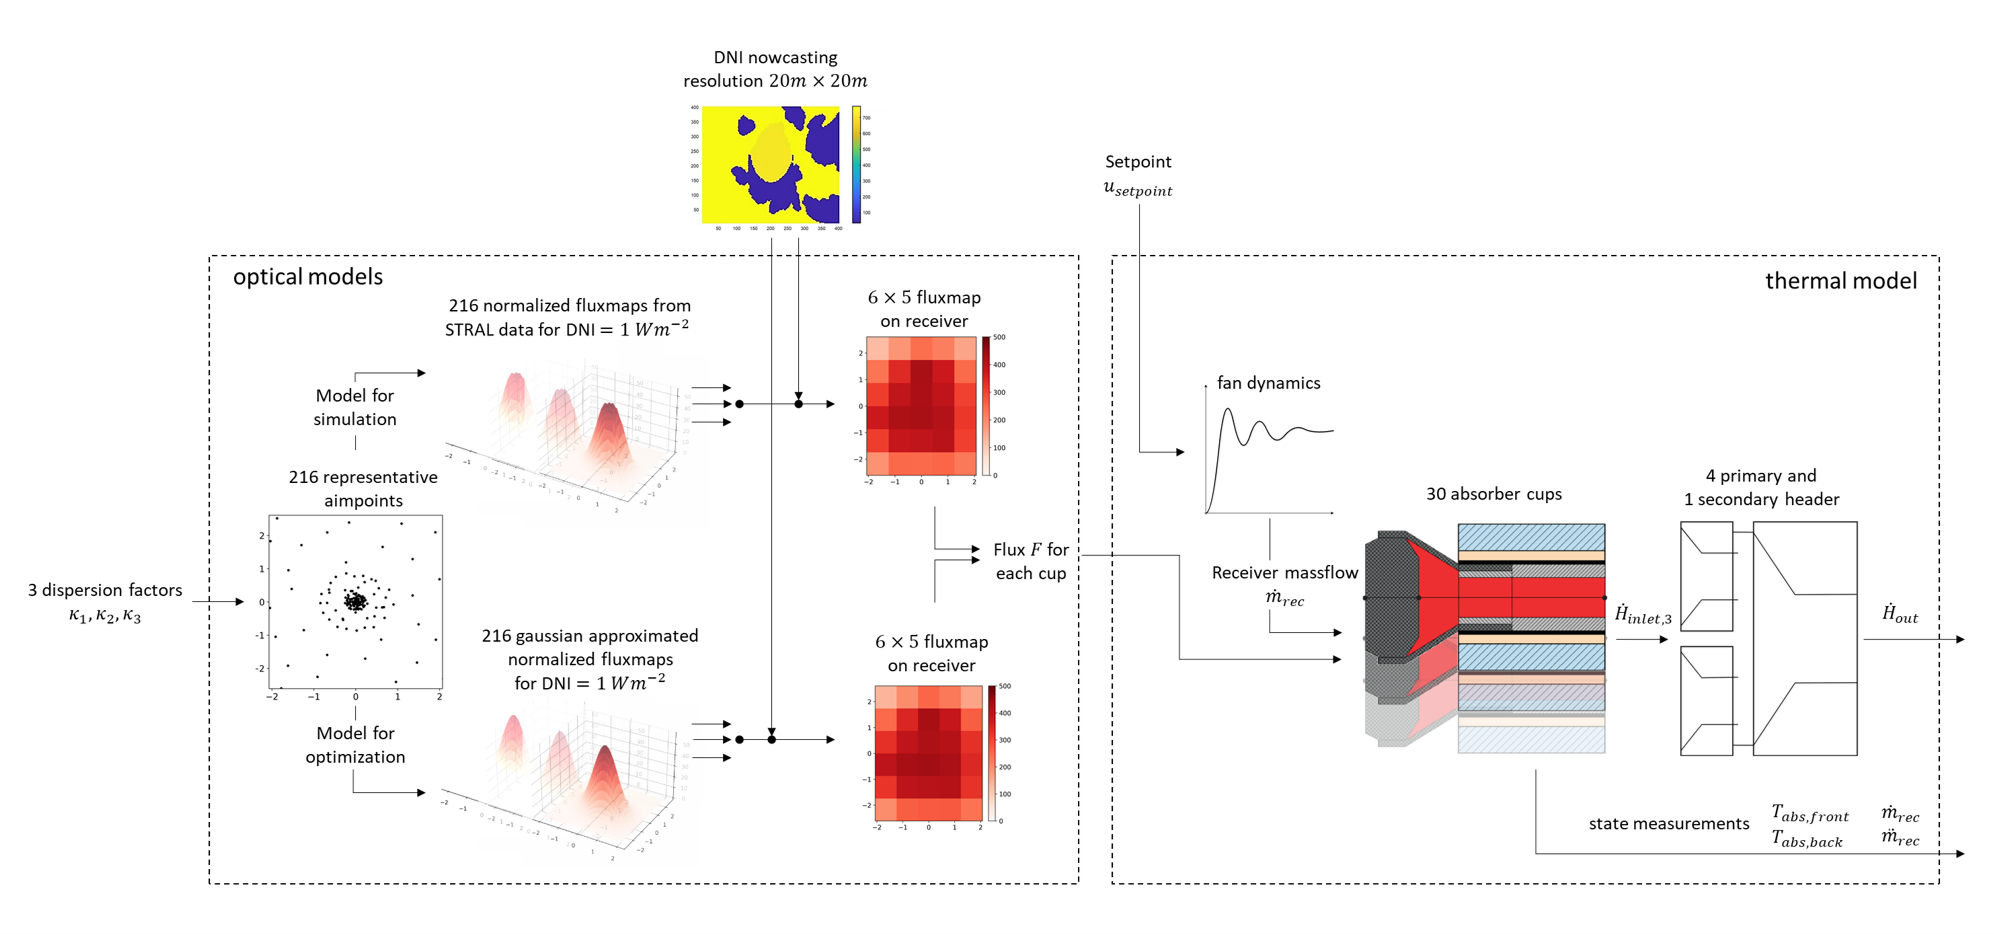
\includegraphics[width=0.98\textheight]{C:/Users/gesc_ma/VSCode MPC Projekt/dynaovrcontroller/dynaovrcontroller/aimpoint_control_scenarios/plots/11_analysis_optical_model/Modellbildung.png}}}
    \caption[Visualisierung der wesentlichen Schritte der Modellbildung]{Visualisierung der wesentlichen Schritte der Modellbildung}
    \label{fig_ZusammenfassungKopplung}
\end{figure}

Es ist erkennbar, dass zwei unterschiedliche optische Modelle entstehen.
Eines, welches Simulatitonszwecken dient und auf mit STRAL berechneten normierten Einstrahlungskarten basiert.
Das zweite Modell nutzt approximierte normierte Einstrahlungskarten, um den Rechenaufwand in dem Optimierungsproblem zu verringern.
Durch diese Einstrahlungskarten wird in beiden optischen Modellen die Flussdichteverteilung auf dem Receiver für $\SI{6}{} \times \SI{5}{}$ Cups anhand von drei Streuungsfaktoren $\kappa$ und dem lokalen DNI-Wert beschrieben.\\
Die Eingangsgrößen des thermischen Modells sind die Flussdichte auf jedem der 30 Absorbercups und der Einstellwert $u_{\mathrm{setpoint}}$ für die Gebläse/Ventil-Kombination.
Durch $62$ Differentialgleichungen und $60$ algebraische Gleichungen ergibt sich der Enthalpiestrom der Luft am Receiveraustritt $\dot{H}_{\mathrm{out}}$ und die Fronttemperatur des Receivers $\TAbsorberFront$ sowie alle weiteren Zustandsmesswerte.

